\documentclass[12pt,a4paper]{article}

%% ── Packages ──────────────────────────────────────────────────────────────
\usepackage[a4paper, margin=2.5cm]{geometry}
\usepackage{amsmath,amssymb,amsfonts}
\usepackage{graphicx}
\usepackage{booktabs}
\usepackage{array}
\usepackage{tabularx}
\usepackage{longtable}
\usepackage{multirow}
\usepackage{hyperref}
\usepackage{setspace}
\usepackage{newunicodechar}
\newunicodechar{₂}{$_2$}
\usepackage{parskip}
\usepackage{enumitem}
\usepackage{caption}
\usepackage{subcaption}
\usepackage{float}
\usepackage[patch=none]{microtype}
\usepackage{algorithm}
\usepackage{algpseudocode}
\usepackage{mathtools}
\usepackage{bm}
\usepackage{titlesec}
\usepackage{fancyhdr}
\setlength{\headheight}{15pt}
\usepackage[T1]{fontenc}
\usepackage[utf8]{inputenc}

\hypersetup{colorlinks=false, hidelinks,
  pdftitle={Multi-Objective Quantum-Chemical MOF Recommendation},
  pdfauthor={Soumya Sekhar Banerjee, Arnd Koeppe, Mehrdad Jalali}}

\onehalfspacing
\setlength{\parindent}{0pt}
\setlength{\parskip}{6pt}

\titleformat{\section}{\large\bfseries}{\thesection}{1em}{}
\titleformat{\subsection}{\normalsize\bfseries}{\thesubsection}{1em}{}
\titleformat{\subsubsection}{\normalsize\bfseries}{\thesubsubsection}{1em}{}

\captionsetup{font=small,labelfont=bf,format=plain,justification=justified}

\pagestyle{fancy}
\fancyhf{}
\fancyhead[L]{\small\textit{QMOF-Rec: Multi-Objective MOF Recommendation}}
\fancyhead[R]{\small\thepage}
\renewcommand{\headrulewidth}{0.4pt}

\newcolumntype{L}[1]{>{\raggedright\arraybackslash}p{#1}}
\newcolumntype{C}[1]{>{\centering\arraybackslash}p{#1}}
\newcolumntype{R}[1]{>{\raggedleft\arraybackslash}p{#1}}

\begin{document}

%% ── Title ─────────────────────────────────────────────────────────────────
\hypersetup{pageanchor=false}
\begin{titlepage}
\centering\vspace*{1cm}
{\LARGE\bfseries QMOF-Rec: A Multi-Objective Recommender-System Framework for Quantum-Chemical MOF Candidate Screening\par}
\vspace{1.2cm}
{\large Soumya Sekhar Banerjee$^{1}$,
Arnd Koeppe$^{2,3}$,
Mehrdad Jalali$^{1,*}$\par}
\vspace{0.8cm}
{\normalsize
$^{1}$ SRH University of Applied Sciences Heidelberg, Heidelberg, Germany\par
$^{2}$ Karlsruhe Institute of Technology (KIT), Institute for Applied Materials - Microstructure Modeling and Simulation (IAM-MMS), Karlsruhe, Germany\par
$^{3}$ Karlsruhe Institute of Technology (KIT), Institute of Nanotechnology - Microstructure Simulation (INT-MSS), Karlsruhe, Germany\par
$^{*}$ Corresponding author: Mehrdad Jalali; Email: mehrdad.jalali@srh.de\par}
\vspace{1cm}
\begin{abstract}
\small\singlespacing\noindent
QMOF-Rec formulates screening of existing metal--organic framework records as query-conditioned top-$K$ recommendation under incomplete metadata. Its contribution is a system-level formulation that separates masked utility scoring, material-space diversity, candidate generation, and auxiliary explanation; it does not introduce a new general-purpose optimizer or generate new materials. A reproducible evaluation uses 20{,}372 records, five query scenarios, ten seeds, and shared candidate pools. Density is complete, band gap is observed for 10{,}810 records, and unavailable void fraction is excluded. WeightedSum, TOPSIS, MMR, and LEA tie on Rel@5=0.8479 and NDCG@5=1.0000 because these metrics use the same utility that WeightedSum sorts. Hybrid diversity is 0.0187 for WeightedSum, 0.0224 for LEA, and 0.0241 for MMR. A joint sensitivity sweep separates the gamma term from the redundancy penalty; disabling both yields diversity 0.0187. An added differential-evolution portfolio baseline reaches diversity 0.0242 and Rel@5=0.8479. Correcting MMR to stop at five selections preserves its output and makes it faster than LEA, so the earlier LEA runtime advantage is not retained. Descriptor-level checks characterize screening behavior without claiming adsorption, experimental, or new DFT validation. Explanation remains auxiliary; deterministic template outputs are not an independent LLM-quality benchmark.
\par\medskip\noindent\textbf{Keywords:} QMOF; candidate screening; incomplete metadata; recommendation; diversity; differential evolution
\end{abstract}
\end{titlepage}
\hypersetup{pageanchor=true}

%% ════════════════════════════════════════════════════════════════════════════
\section{Introduction}
\label{sec:intro}

Materials discovery increasingly depends on computational screening, machine learning, and interactive decision support because experimentally accessible materials spaces are too large to explore by manual intuition alone. Metal--organic frameworks (MOFs) are a representative example: their modular chemistry, tunable pore environments, and broad electronic-property landscape make them attractive for gas adsorption, storage, catalysis, separations, sensing, drug delivery, and electronic applications. Yet the same chemical diversity creates a practical recommendation problem.

We present QMOF-Rec, a multi-objective scientific recommender system for quantum-chemical MOF candidate screening. Screening existing QMOF records can be formulated as a scientific top-$K$ recommendation task: given a user query and an incomplete set of material descriptors, the system must return a ranked and diverse shortlist of candidate MOFs that are relevant, scientifically plausible, and useful for follow-up investigation.

In this manuscript, \emph{quantum-chemical MOF recommendation} means recommending experimentally derived QMOF records using query intent together with available quantum-chemical and metadata-derived signals such as band gap, density, stability proxies, and engineered metadata-proxy signals. The formulation extends conventional single-target screening by modelling recommendation as a multi-objective ranking problem over relevance, property suitability, diversity, and engineered metadata-proxy signals.

The Quantum MOF (QMOF) database introduced by Rosen et al.\ provides quantum-chemical properties for experimentally derived MOF structures and has become an important resource for machine-learning-assisted MOF discovery \cite{rosen2021,rosen2022}. However, using QMOF as a recommendation substrate is different from using it as a static table. A scientific recommender must interpret user intent, retrieve a candidate pool, score property suitability, avoid redundant candidates, explain trade-offs, and communicate uncertainty when descriptors are missing. This is especially important for queries such as ``CO$_2$ adsorption MOFs'' or ``photocatalytic MOFs'', where semantic relevance alone is not equivalent to scientific suitability.

QMOF recommendation is a query-conditioned candidate-prioritization problem rather than a database lookup. A user rarely asks only for the nearest textual match to a query; instead, they seek a scientifically plausible portfolio of candidates that balances several objectives under incomplete evidence. Vector retrieval can identify materials whose metadata are textually or semantically related to a query, but semantic similarity alone is not a sufficient scientific objective. A material may match a query textually while lacking the available band-gap, density, stability-proxy, or metadata-proxy signals needed for a specific use case. Conversely, a material with sparse metadata may remain worth inspecting when its observed descriptors or formula-derived metadata proxies resemble high-value candidates. QMOF recommendation is therefore naturally multi-objective and partially evidence-limited.

The central idea of QMOF-Rec is to use retrieval for candidate generation, property and metadata-proxy scoring for scientific item representation, LEA-guided optimization for multi-objective top-$K$ portfolio construction, and candidate-conditioned interaction for explainable recommendation. The implemented evaluation focuses on the LEA-guided reranking layer and deterministic explanation safeguards. The broader architecture includes prospective graph-aware representation learning and property prediction, together with retrieval-augmented assistance and user feedback.

The methodological contribution is the explicit formulation of query-conditioned screening under incomplete metadata: utility scoring uses observation masks, diversity is measured in a separate full-precision material representation, and explanation is separated from selection. These choices make assumptions and trade-offs auditable. The constituent retrieval, masking, evolutionary search, and graph-learning ideas are established methods; LEA is one evaluated reranking policy, not the core novelty. Its diversity lies between WeightedSum and MMR in the reproduced setting, but the corrected top-five runtime comparison does not support preferring LEA over MMR.

The contributions are:
\begin{enumerate}[leftmargin=*,label=\arabic*.]
\item A query-conditioned screening formulation for existing QMOF records that distinguishes observed, missing, and heuristic information.
\item A separation of masked recommendation utility from full-precision material diversity, exposing the loss of resolution caused by binned score distances.
\item An empirical characterization of reranking trade-offs using shared pools, scenario-level analysis, component ablations, coefficient sensitivity, and a differential-evolution portfolio comparator.
\item An auditable separation of ranking evidence from auxiliary explanation and prospective learned representations, with explicit limits on physical validation.
\end{enumerate}

%% ════════════════════════════════════════════════════════════════════════════
\section{QMOF-Rec as a Scientific Recommender System}
\label{sec:rec}

QMOF-Rec is designed as a query-driven scientific recommender system. The user is a materials scientist, chemist, or researcher seeking a practical shortlist of candidate MOFs for a target application. The items are QMOF material records. The user intent is expressed as a scientific query such as ``CO$_2$ adsorption MOFs'', ``photocatalytic MOFs'', ``lightweight storage frameworks'', or ``wide-band-gap insulating frameworks''. The recommendation task is to map this query context to a top-$K$ list of QMOF candidates that balances relevance, scientific suitability, diversity, and available engineered metadata proxies.

The architecture follows a common two-stage recommender-system design. Candidate generation first narrows the searchable item universe to a query-relevant candidate pool using vector, semantic, or metadata retrieval. Ranking and reranking then operate on this smaller candidate set. Deterministic rankers such as WeightedSum, Technique for Order Preference by Similarity to Ideal Solution (TOPSIS), ParetoCrowding, SemanticOnly, Random, and maximal marginal relevance (MMR) provide baseline recommendation policies, while LEA-guided multi-objective reranking optimizes the final user-facing top-$K$ candidate portfolio. Explanation is provided through candidate-conditioned recommendation rationale, uncertainty communication, and evidence-grounded response generation.

Table~\ref{tab:rec_mapping} makes explicit that QMOF-Rec is a hybrid scientific recommender with a strong content-based focus rather than a collaborative-filtering system. No large-scale user--MOF interaction matrix is currently available. Instead, recommendation is driven by query context and item content, including metadata, property scores, semantic retrieval signals, and engineered metadata-proxy representations.

\begin{table}[H]
\centering
\caption{Mapping classical recommender-system components to QMOF-Rec.}
\label{tab:rec_mapping}
\small
\begin{tabular}{L{2.8cm} L{4.5cm} L{5.5cm}}
\toprule
\textbf{RS Concept} & \textbf{QMOF-Rec Implementation} & \textbf{Role in Candidate Screening}\\
\midrule
User & Materials scientist, chemist, or researcher & Defines scientific intent and evaluates usefulness\\
Item & QMOF material candidate & Candidate MOF for follow-up investigation\\
Query/context & Application-oriented scientific query & Specifies target use case and objective weights\\
Candidate generation & Vector, semantic, or metadata retrieval & Narrows QMOF search space to $C_q$\\
Item representation & Metadata, formula, density, band gap, stability proxy, metadata proxies, semantic metadata & Encodes scientific signals for ranking\\
Scoring function & Query-dependent objective utility & Estimates relevance and suitability\\
Multi-objective ranking & WeightedSum, TOPSIS, ParetoCrowding, SemanticOnly, Random, MMR & Provides deterministic and diversity-aware baselines\\
Reranking & LEA-guided multi-objective reranking & Optimizes final top-$K$ portfolio\\
Top-$K$ recommendation & Ranked shortlist $S_K(q)$ & Produces practical candidate list for expert inspection\\
Diversity & Intra-list diversity and future novelty metrics & Reduces redundant candidate portfolios\\
Explanation & Candidate-conditioned rationale and uncertainty explanation & Supports interpretable scientific decision support\\
Feedback & User/expert feedback, logging, analytics & Enables future preference-aware improvement\\
\bottomrule
\end{tabular}
\end{table}

%% ════════════════════════════════════════════════════════════════════════════
\section{Related Work}
\label{sec:related}

\subsection{QMOF Databases and Machine-Learning-Assisted MOF Discovery}

High-throughput computational databases have reshaped materials informatics by making electronic, structural, and thermodynamic properties available at scales that support statistical learning. QMOF is especially relevant because it focuses on quantum-chemical properties of MOFs and coordination polymers \cite{rosen2021}. Rosen et al.\ later expanded the electronic-property analysis of QMOF and benchmarked graph neural networks for high-throughput electronic-property prediction \cite{rosen2022}. These studies establish QMOF as a resource for property prediction, screening, and data exploration.

Machine learning has also been used broadly for materials and MOF screening, including adsorption-property prediction, band-gap prediction, and data-driven discovery workflows. Seko et al.\ demonstrated that matrix- and tensor-based recommender systems can prioritize currently unknown inorganic compounds \cite{seko2018}. Transformer-based MOF representations such as MOFormer illustrate the increasing role of learned representations for QMOF and hypothetical MOF tasks \cite{luo2023}. Recent natural-language-guided materials discovery work further motivates query-conditioned retrieval and ranking interfaces for scientific users \cite{qu2023}. In the present work, QMOF records are used as the retrieval and recommendation substrate. Because the locally available metadata are incomplete for some descriptors, the manuscript avoids strong adsorption-specific claims and focuses on ranking behavior under the descriptors actually present.

\subsection{Graph-Based and Structure-Aware MOF Learning}

Graph neural networks (GNNs) are natural for molecular and crystalline materials because atoms, bonds, distances, and higher-level material relationships can be represented as nodes, edges, and attributes. Crystal Graph Convolutional Neural Networks (CGCNN) demonstrated interpretable graph-based prediction of crystalline properties \cite{xie2018}. Graph networks have also been framed as a general machine-learning architecture for molecules and crystals \cite{chen2019}. Foundational GNN methods include the graph convolutional network (GCN) \cite{kipf2017}, GraphSAGE \cite{hamilton2017}, and Graph Attention Networks (GAT) \cite{velickovic2018}.

MOF-specific graph learning has developed rapidly. MOFGalaxyNet used social-network-style graph analysis and graph convolutional learning to predict guest accessibility in MOFs \cite{jalali2023}. The Black Hole Strategy later introduced gravity-based representative sampling for frugal graph learning on MOF networks, including GraphSAGE, GCN, and GAT experiments \cite{jalali2025bh}. These works motivate the graph-aware extension in QMOF-Rec: learned graph embeddings can provide relational signals in future extensions; the evaluated ranking signals below are engineered metadata proxies.

\subsection{Retrieval-Augmented Systems and Vector Search}

Large-scale vector retrieval enables fast nearest-neighbor search over embedded documents, materials, and metadata. FAISS is a widely used library for billion-scale similarity search \cite{johnson2019}. Sentence-BERT showed that Siamese sentence-transformer architectures can produce effective dense sentence embeddings for semantic search \cite{reimers2019}. Retrieval-Augmented Generation (RAG) combines parametric generation with retrieved evidence to support knowledge-intensive tasks \cite{lewis2020}.

For QMOF-Rec, retrieval serves two functions. First, it provides a candidate pool for recommendation. Second, it supplies evidence for the scientific assistant. The LLM is treated as an explanation and interaction layer rather than as a source of ground-truth material properties. This distinction is important because generated text can be fluent while still requiring verification against QMOF metadata, retrieved literature, and candidate records.

The deployed repository separates semantic retrieval from numerical reranking. Retrieval uses SentenceTransformer embeddings of metadata text templates stored in a FAISS L2 index; it does not search directly over the normalized numerical objective vector used by WeightedSum or LEA. During vector-index construction, unavailable fields are serialized as unavailable metadata rather than numerical zeros. Reranking then constructs explicit objective vectors and availability masks for semantic score, band-gap score, density score, and stability score. The reproducible offline benchmark tables were generated with a deterministic semantic proxy over metadata text and formula tokens rather than by rerunning a live sentence-embedding search.

Research-data assistants such as KadiAssistant provide a related but distinct direction: privacy-preserving access to heterogeneous research repositories through semantic search and local or self-hosted language-model components \cite{kadiassistant2026}. QMOF-Rec instead focuses on MOF candidate retrieval, objective-aware reranking, and recommendation evaluation over QMOF-derived metadata.

\subsection{Scientific, Content-Based, and Hybrid Recommender Systems}

Scientific recommender systems extend classical recommendation from consumer preference prediction to expert decision support, candidate discovery, and prioritization under incomplete evidence. In materials discovery, Seko et al.\ used matrix- and tensor-based recommender systems to identify currently unknown inorganic compounds \cite{seko2018}, and Qu et al.\ used language representations for materials exploration and discovery \cite{qu2023}. In QMOF-Rec, users are scientists and items are material candidates rather than products, movies, or documents. The absence of large user--item interaction histories makes the problem closer to query-driven, content-based, context-aware recommendation than to collaborative filtering. Content-based recommenders rank items using item attributes and user/query profiles, while hybrid recommenders combine multiple signals such as metadata, semantic retrieval, graph representations, and user feedback when available \cite{burke2002,lops2011,ricci2011}.

QMOF-Rec is therefore a query-driven hybrid recommender with a strong content-based focus. Candidate items are represented by QMOF metadata, formula-derived information, property scores, engineered metadata proxies, and semantic retrieval signals. This differs from matrix/tensor completion over composition spaces \cite{seko2018} and complements language-representation-based material ranking \cite{qu2023} by adding descriptor masks, metadata-proxy augmentation, and LEA list-level reranking. Future user feedback can support preference-aware or online recommendation, but the current offline evaluation uses query-dependent objective weights rather than click logs or explicit ratings.

\subsection{Multi-Objective Recommender Systems and Diversity-Aware Reranking}

Scientific recommendation is typically a multi-objective problem. Candidate portfolios should include relevant, diverse, and non-redundant materials rather than a list of nearly identical top-scoring records. Multi-criteria recommender systems explicitly model multiple utility dimensions \cite{adomavicius2011,jannach2014}, while explainable recommendation emphasizes transparency and user trust \cite{zhang2020}. Diversity-aware reranking has a long history in information retrieval, including maximal marginal relevance (MMR) \cite{carbonell1998}.

Classical decision methods also remain useful baselines. TOPSIS ranks alternatives by closeness to ideal and anti-ideal solutions \cite{hwang1981}. Pareto ranking and crowding-distance strategies provide diversity-aware approximations of multi-objective selection, and Non-dominated Sorting Genetic Algorithm II (NSGA-II) is a standard evolutionary reference method for multi-objective optimization \cite{deb2002}. QMOF-Rec evaluates weighted-sum, TOPSIS, ParetoCrowding, random, semantic-only, and LEA-based reranking under a common top-$K$ protocol.

Unlike similarity-only material recommendation, QMOF-Rec formulates MOF candidate screening as a multi-objective top-$K$ recommendation problem. It combines retrieval augmentation, property-aware scoring, engineered metadata proxies, LEA-guided reranking, and explanation support to recommend diverse candidate portfolios rather than only nearest-neighbor materials.

\subsection{Explainable Recommendation and Scientific Assistance}

Explainable recommender systems aim to clarify why items are recommended, how scores are produced, and where uncertainty remains \cite{zhang2020}. For scientific recommendation, explanation is especially important because candidate lists may influence costly follow-up experiments, simulations, or synthesis decisions. In QMOF-Rec, candidate-conditioned explanations are framed as an explainable-recommendation layer that can summarize retrieved evidence, material metadata, objective trade-offs, and uncertainty flags. The current manuscript does not claim that LLM explanation improves recommendation accuracy, and live-LLM faithfulness remains a separate future evaluation target.

\subsection{Nature-Inspired and Evolutionary Optimization for Scientific Discovery}

Nature-inspired and evolutionary optimization methods are often used when search spaces are continuous, nonconvex, or multi-objective. Particle swarm optimization, genetic algorithms, NSGA-II, and related evolutionary or swarm-based methods have been applied across scientific discovery and engineering optimization \cite{deb2002}. Bayesian optimization is better described separately as model-based sequential optimization for expensive black-box objectives \cite{shahriari2016}. The Lotus Effect Algorithm (LEA) is a lotus-nature-inspired optimization algorithm originally proposed for engineering design optimization \cite{dalirinia2024}. MOF-LENS later used LEA-inspired optimization for accelerated discovery of MOF nanocarriers for doxorubicin delivery \cite{jalali2025lens}.

The present work distinguishes the original LEA algorithm from the implemented LEA-rec adaptation. LEA-rec uses lotus-inspired mutation and self-cleaning replacement in a post-retrieval normalized objective space, then maps candidates back to valid QMOF records. The method constructs recommendation portfolios from a retrieved candidate pool and leaves physics-based validation, DFT, adsorption simulations, and expert assessment as downstream steps.

\subsection{Positioning of the Present Work}

This manuscript positions QMOF-Rec between materials informatics, recommender systems, graph learning, and scientific-assistant systems. It models user intent and top-$K$ recommendation, evaluates candidates using objective scores and diversity, and grounds explanations in retrieved evidence and material metadata. The evaluated graph-named variants are engineered metadata proxies; trained metadata-graph, CIF-derived, and atomistic GNN comparisons remain future work.

%% ════════════════════════════════════════════════════════════════════════════
\section{End-to-End QMOF-Rec Recommendation Workflow}
\label{sec:arch}

QMOF-Rec is framed as an end-to-end workflow for screening existing material records. Figure~\ref{fig:qmof_workflow} separates the executed offline benchmark from prospective learned-representation and validation extensions. The executed workflow uses query-dependent candidate generation, masked active objectives, engineered metadata proxies, ranking and reranking, a top-five shortlist, and auxiliary explanation templates.

\begin{figure}[H]
  \centering
  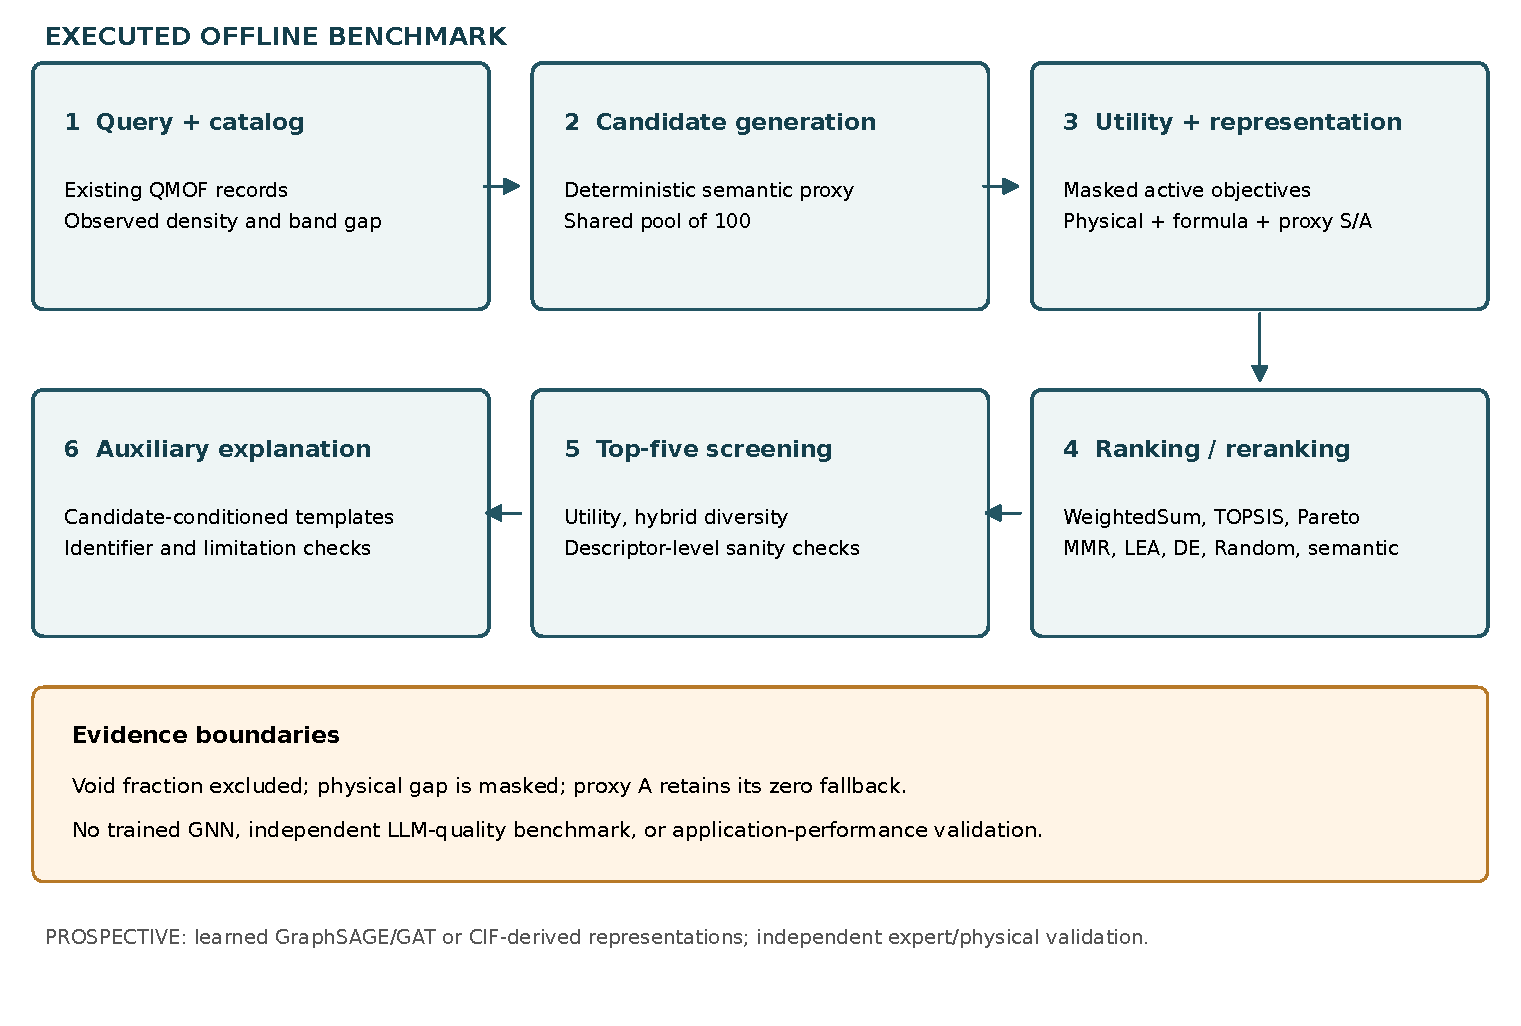
\includegraphics[width=0.99\textwidth]{figures/workflow_metadata_proxies.pdf}
  \caption{Executed offline screening workflow and explicitly separate prospective extensions. Candidate generation uses the deterministic semantic proxy; current representation augmentation uses engineered metadata proxies S and A, not trained graph embeddings. Masks apply to active objectives and physical coordinates; proxy A retains the disclosed missing-gap fallback. Explanation templates are auxiliary and do not change rankings.}\label{fig:qmof_workflow}
\end{figure}

\subsection{Scientific Query and Candidate Representation}

The workflow starts from a scientific query and QMOF metadata. Query text, formula tokens, and available material descriptors are converted into text and metadata representations for semantic candidate retrieval. This retrieval stage generates the candidate pool used by all downstream rankers, so the final comparison is conditioned on a shared set of query-relevant QMOF records rather than the full catalog.

Each retrieved candidate has masked active objectives and masked physical coordinates. The engineered proxy-A coordinate separately retains the missing-gap fallback disclosed in Section~\ref{sec:graph}. Availability masks prevent missing physical coordinates from being interpreted as measured zeros; in particular, void fraction is excluded from numerical ranking because it is unavailable in the evaluated metadata. Objective-space scoring and portfolio-level hybrid material diversity are kept distinct: active objective scores support relevance and suitability scoring, while the hybrid material representation supports list-level diversity comparisons.

The executed representation uses engineered formula/descriptor metadata proxies. Learned metadata graphs or atomistic representations are prospective extensions. The current proxy values do not validate adsorption, synthesizability, or industrial readiness. WeightedSum, TOPSIS, and MMR provide comparison methods, while LEA performs multi-objective reranking over the retrieved candidate pool to produce the final top-$K$ recommendation portfolio.

Candidate-conditioned explanations are generated from retrieved records, available descriptors, scores, and missing-descriptor warnings. They are designed to communicate objective trade-offs and limitations while preserving safeguards against unsupported claims. The deterministic routine below checks only identifier inclusion and limitation phrases; assigned flags do not independently establish safeguard behavior.

\subsection{Interface Demonstration}

The interface prototype was executed locally and inspected through browser-based screenshots (Figure~\ref{fig:frontend}). These views demonstrate how the recommendation workflow can be exposed to a user through query input, scientific chat, recommendation, material-inspection, and analytics views. The screenshots are illustrative interface evidence and do not replace the offline ranking, metadata-proxy, ablation, or deterministic candidate-conditioned explanation evaluations.

\begin{figure}[H]
  \centering
  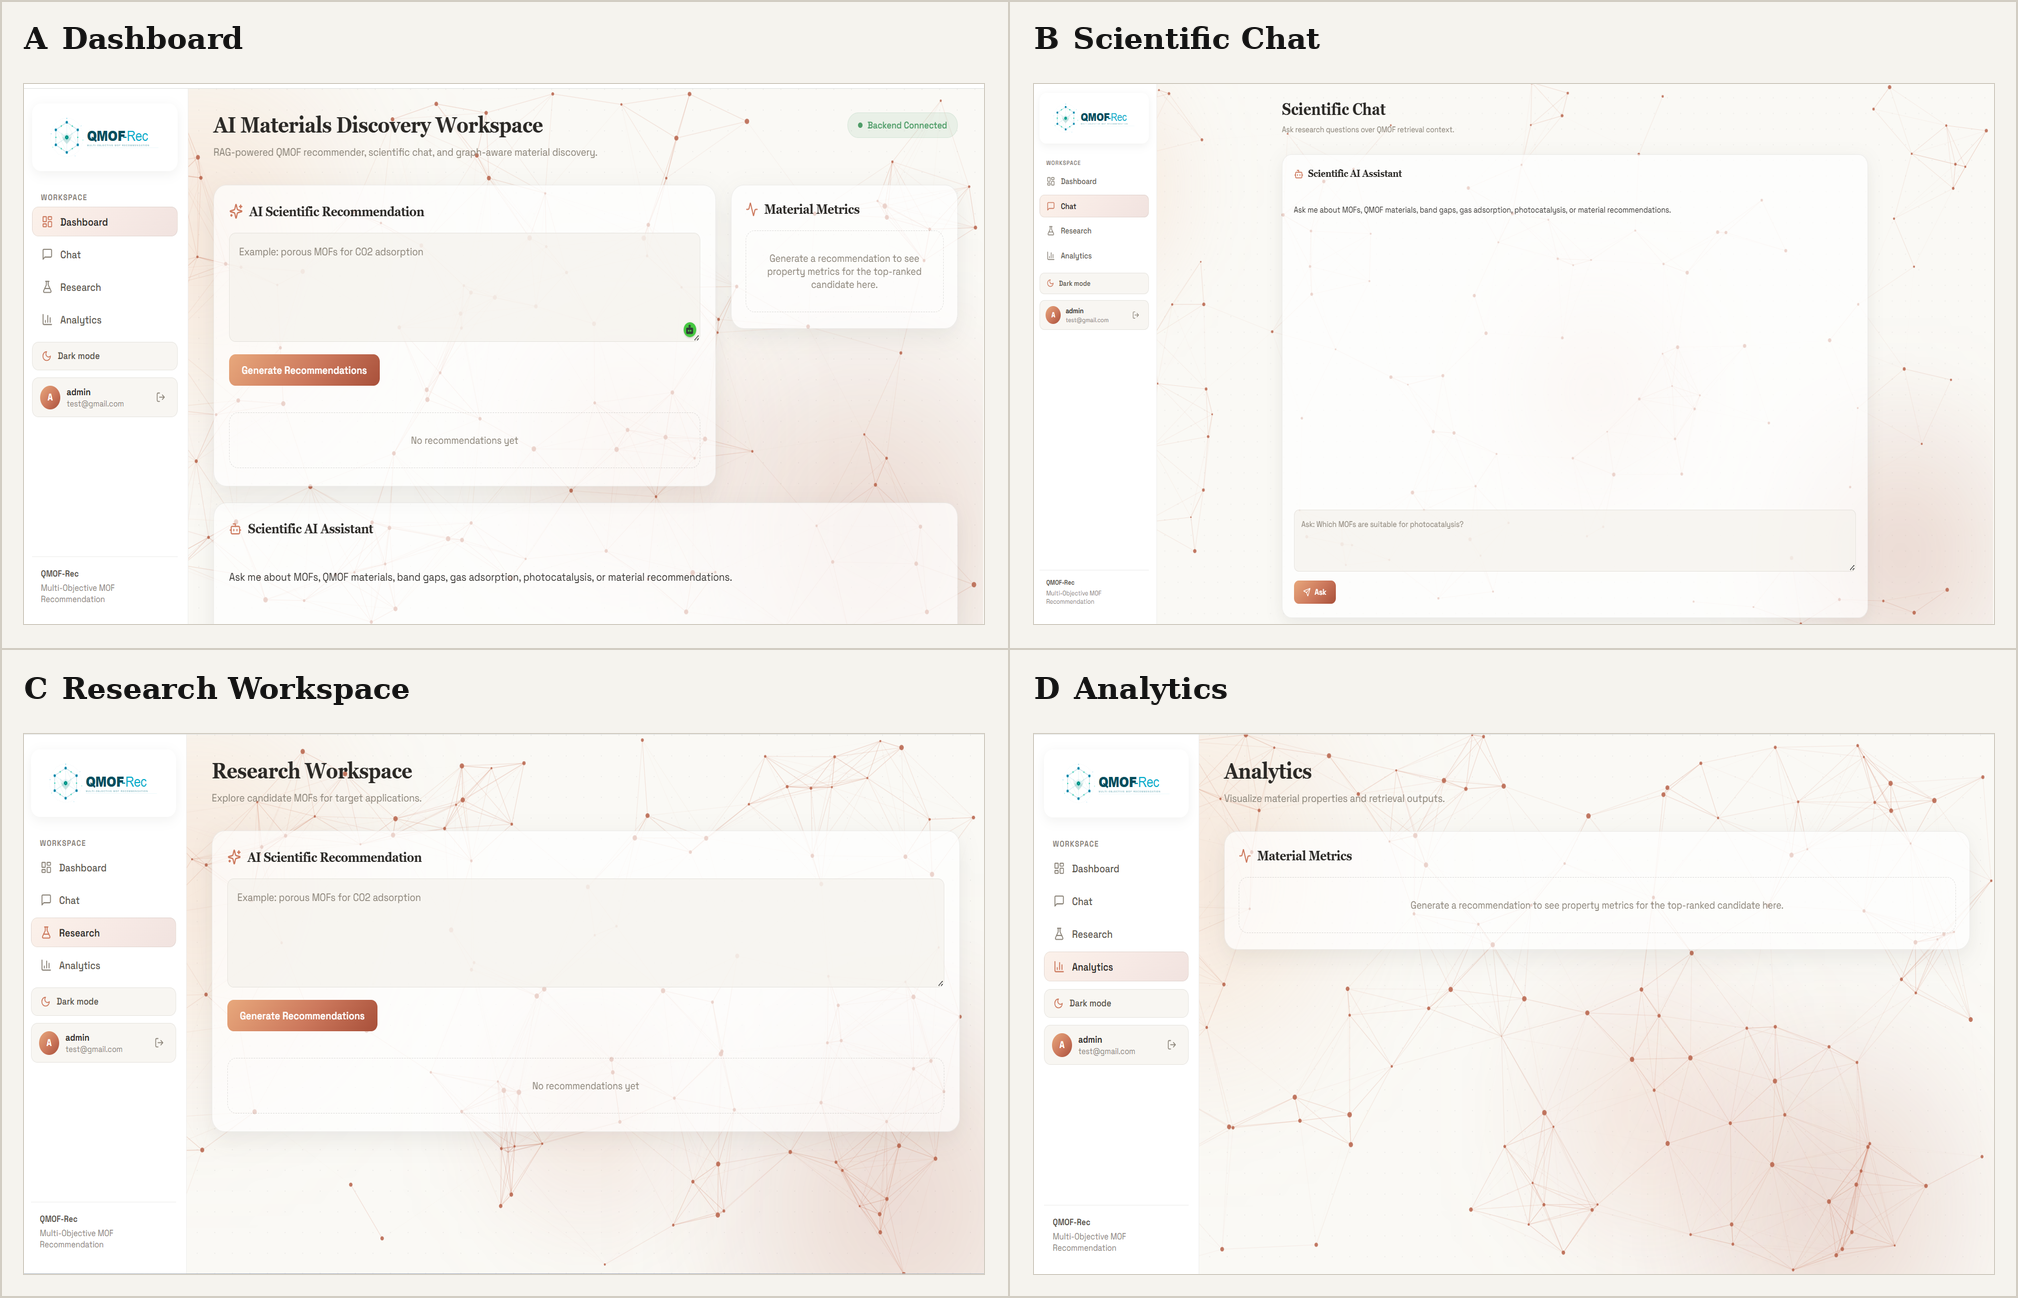
\includegraphics[width=0.85\linewidth]{figures/fig2_qmof_frontend.png}
  \caption{Compact QMOF-Rec application screenshot montage. Panel~A shows the recommendation workspace, Panel~B the scientific chat interface, Panel~C the research workspace, and Panel~D the analytics view. Screenshots demonstrate the implemented interface and are not part of the offline ranking validation.}
  \label{fig:frontend}
\end{figure}

%% ════════════════════════════════════════════════════════════════════════════
\section{End-to-End Recommendation Scenario}
\label{sec:scenario}

This section illustrates how QMOF-Rec operates as a scientific recommender system from user request to final recommendation. Consider a materials scientist who enters the query: ``Recommend promising MOFs for CO$_2$ adsorption with low density and good stability.'' QMOF-Rec treats this input as a recommendation context rather than only as a text-search string. The system identifies semantic relevance to CO$_2$ adsorption, density, stability proxy, diversity, and optional metadata-proxy scores as relevant objectives. Because void fraction is unavailable in the current metadata, porosity is not used as an active numerical objective.

The first stage is candidate generation. QMOF-Rec retrieves an initial candidate pool $C_q$ from the QMOF metadata/vector store. This stage is analogous to candidate generation in a two-stage recommender-system pipeline: it narrows the full QMOF item catalog to a smaller set of query-relevant materials. In the current reproducible evaluation, this pool contains 100 candidate QMOF records for each query scenario.

Each retrieved material is then represented as an item feature vector. Available descriptors and scores, including formula-derived signals, density, band gap where available, semantic metadata score, stability proxy, and metadata-derived objective scores, are normalized before ranking. Missing descriptors are handled explicitly. In particular, void fraction is absent in the current metadata, so the system avoids strong adsorption or porosity claims and communicates that limitation in the recommendation rationale.

The current benchmark can augment scoring with engineered metadata proxies S and A. A separate prospective extension could use learned GraphSAGE/GAT or CIF-derived representations; none is trained or evaluated in the final ranking protocol.

The retrieved pool can be ranked by multiple baselines. WeightedSum provides the strongest relevance-oriented scoring baseline. TOPSIS ranks candidates by distance to ideal and anti-ideal solutions. ParetoCrowding emphasizes trade-offs and diversity. MMR provides a diversity-aware reranking reference. SemanticOnly and Random provide retrieval-only and chance-level controls. LEA is the active multi-objective reranker. In recommender-system terms, LEA acts as a multi-objective reranker whose diversity effect depends on the resolution and geometry of the selected material representation.

Table~\ref{tab:workflow} summarizes the complete workflow. The final output is a ranked top-$K$ list in which each recommendation can include the QMOF identifier, formula, available property values, method score, a short rationale, and a warning when relevant descriptors are missing. The auxiliary explanation routine is audited in Section~\ref{sec:rag_eval}; assigned scores are not independent quality evidence, and explanation does not alter ranking. After inspecting candidate records or 3D/CIF structures where available, the user can mark materials as useful, uncertain, or irrelevant. Such feedback is stored for future expert review and possible preference-aware recommendation.

\begin{table}[H]
\centering
\caption{Example end-to-end QMOF-Rec recommendation scenario.}
\label{tab:workflow}
\small
\begin{tabular}{L{2.2cm} L{3.4cm} L{2.8cm} L{4.3cm}}
\toprule
\textbf{Step} & \textbf{System Action} & \textbf{RS Role} & \textbf{QMOF-Rec Output}\\
\midrule
User query & Interpret ``CO$_2$ adsorption with low density and good stability'' & Query/context capture & Weights for relevance, density, stability, diversity, and metadata-proxy signal; porosity excluded when void fraction is unavailable\\
Candidate generation & Retrieve 100 query-relevant QMOF records & First-stage candidate generation & Candidate pool $C_q$\\
Objective scoring & Normalize available descriptors and metadata scores & Item representation and scoring & Objective matrix $X_q$ with missing-descriptor flags\\
Metadata proxies & Engineered formula/descriptor metadata proxies & Current benchmark & Proxy S and proxy A augmentation\\
Prospective learning & Learned GraphSAGE/GAT or CIF-derived representations & Future extension & Not executed in the benchmark\\
Baseline ranking & Apply deterministic and diversity-aware policies & Baseline top-$K$ ranking & Comparable ranked lists for offline evaluation\\
LEA reranking & Optimize relevance, balance, and diversity & List-level reranking & LEA-guided top-$K$ portfolio\\
Top-$K$ output & Return ranked QMOF candidates & User-facing recommendation & IDs, formulas, values, scores, and warnings\\
Explanation & Generate evidence-aware rationale & Explainable recommendation & Trade-off and uncertainty notes\\
Feedback & Record expert judgments & Future preference learning & Logs for review and later preference modeling\\
\bottomrule
\end{tabular}
\end{table}

Table~\ref{tab:co2_example} reports the final diversity-aware, mask-aware LEA top-5 recommendation output for the CO$_2$ adsorption scenario from the rerun artifact directory \path{artifacts/final_diversity_aware_masked_protocol/rankings}. The values should be interpreted under the metadata limitations above: density and band-gap values are available for these records, but void fraction is unavailable. Candidate ties in active utility scores are broken by the LEA fitness, which includes the selected diversity representation and the seed-dependent candidate-pool order.

\begin{table}[H]
\centering
\caption{Example top-$K$ recommendations for the CO$_2$ adsorption scenario from the final diversity-aware, mask-aware rerun. Void-fraction values are unavailable in the current metadata. Scores are LEA optimization utilities, not probabilities.}
\label{tab:co2_example}
\small
\begin{tabular}{C{1.1cm} L{2.5cm} L{3.9cm} C{1.5cm} C{1.7cm} C{1.9cm}}
\toprule
\shortstack{\textbf{Rank}} & \textbf{QMOF ID} & \textbf{Formula} & \textbf{Density} & \shortstack{\textbf{Band}\\\textbf{gap}} & \shortstack{\textbf{LEA}\\\textbf{score}}\\
\midrule
1 & qmof-82fb334 & Co$_2$C$_{22}$H$_{16}$N$_4$O$_{10}$ & 1.773 & 2.754 & 0.847108\\
2 & qmof-ba8d316 & Co$_2$C$_{32}$H$_{24}$O$_{12}$ & 1.746 & 1.250 & 0.803574\\
3 & qmof-54f7ee7 & Co$_2$K$_2$C$_{48}$H$_{44}$N$_4$O$_6$ & 1.497 & 1.505 & 0.803149\\
4 & qmof-ec84fcf & Co$_2$C$_{20}$H$_{16}$N$_{28}$ & 1.767 & 2.596 & 0.801944\\
5 & qmof-330a403 & {\tiny Co$_2$C$_{58}$F$_{12}$H$_{32}$N$_8$O$_8$S$_2$} & 1.415 & 2.471 & 0.801803\\
\bottomrule
\end{tabular}
\end{table}

The CO$_2$ scenario ranks candidates by balancing query relevance, density, band-gap-derived suitability, and stability proxy values under the available metadata. The missing void-fraction descriptor means these entries should be treated as recommendation candidates for expert follow-up rather than validated CO$_2$ uptake materials.

%% ════════════════════════════════════════════════════════════════════════════
\section{Problem Formulation}
\label{sec:formulation}

Let $\mathcal{M} = \{m_1, \ldots, m_{|\mathcal{M}|}\}$ denote the item catalog of QMOF material records and let $q$ denote a scientific query. In recommender-system terms, $q$ is the query context, $m_i$ is an item, and the goal is to return a ranked top-$K$ recommendation list. The initial candidate-generation stage returns a query-dependent candidate pool
\begin{equation}
  C_q = \{m_1, \ldots, m_n\} \subset \mathcal{M}.
  \label{eq:cq}
\end{equation}
Each candidate item $m_i$ is represented by a normalized active objective vector $\mathbf{x}_i \in [0,1]^d$ and an availability mask $\mathbf{a}_i \in \{0,1\}^d$. The mask entry $a_{ij}=1$ only when objective $j$ is observed or defensibly derived for material $m_i$; unsupported or missing descriptors have $a_{ij}=0$ and are excluded from active numerical scoring. This distinction prevents missing descriptors from being interpreted as physical zero values.
The query-specific weight vector is
\begin{equation}
  \mathbf{w}_q = (w_{q1}, \ldots, w_{qd}),\quad w_{qj} \geq 0,\quad \sum_{j=1}^{d} w_{qj} = 1.
\end{equation}
The objective matrix for the candidate pool is
\begin{equation}
  X_q = \begin{pmatrix} x_{11} & \cdots & x_{1d} \\ \vdots & \ddots & \vdots \\ x_{n1} & \cdots & x_{nd} \end{pmatrix},\quad x_{ij}\in[0,1].
\end{equation}
The corresponding availability matrix is
\begin{equation}
  A_q = \begin{pmatrix} a_{11} & \cdots & a_{1d} \\ \vdots & \ddots & \vdots \\ a_{n1} & \cdots & a_{nd} \end{pmatrix},\quad a_{ij}\in\{0,1\}.
\end{equation}
The recommender outputs a top-$K$ list $S_K \subset C_q$. Let $f(q, m_i, S)$ be the context-aware ranking or reranking utility of item $m_i$ for query $q$, optionally conditioned on the partial recommendation list $S$. The top-$K$ recommendation list is
\begin{equation}
  S_K(q) = \underset{m_i \in C_q}{\operatorname{TopK}}\; f(q, m_i, S).
\end{equation}
For deterministic pointwise rankers, $S$ is ignored. For list-aware reranking, $S$ captures the candidates already selected and enables diversity-aware portfolio construction. The masked weighted relevance score is
\begin{equation}
  R(m_i, q) =
  \frac{\sum_{j=1}^{d} a_{ij}w_{qj}x_{ij}}
       {\sum_{j=1}^{d} a_{ij}w_{qj}}.
  \label{eq:relevance}
\end{equation}
The implementation returns zero when the active-weight denominator is at most $10^{-8}$; otherwise it divides by that denominator without an added epsilon. For a target property $p_i$ and query-specific target $\tau$, a normalized target score can be defined as
\begin{equation}
  s_{\mathrm{target}}(p_i;\tau) = \max\!\left(0, 1 - \frac{|p_i - \tau|}{r + \epsilon}\right),
\end{equation}
where $r$ is a normalization range and $\epsilon$ avoids division by zero. The masked balance score is
\begin{equation}
  B(m_i) =
  \begin{cases}
  1-\sqrt{\dfrac{1}{\sum_j a_{ij}}\displaystyle\sum_{j:a_{ij}=1}\left(x_{ij}-\bar{x}_{i,\mathrm{obs}}\right)^2}, & \sum_j a_{ij} > 0,\\[8pt]
  0, & \sum_j a_{ij}=0.
  \end{cases}
\end{equation}
where $\bar{x}_{i,\mathrm{obs}}$ is the mean of the observed active objectives for candidate $m_i$; the implementation clips this score to $[0,1]$. For two candidates, the joint availability indicator is $a_{i\ell,j}=a_{ij}a_{\ell j}$. Masked cosine similarity is computed only over jointly observed dimensions and is used for auxiliary material-similarity scoring:
\begin{equation}
  \cos_{\mathrm{mask}}(\mathbf{x}_i,\mathbf{x}_\ell)=
  \frac{\sum_{j:a_{i\ell,j}=1}x_{ij}x_{\ell j}}
       {\sqrt{\sum_{j:a_{i\ell,j}=1}x_{ij}^2}\sqrt{\sum_{j:a_{i\ell,j}=1}x_{\ell j}^2}+\epsilon}.
\end{equation}
If no jointly observed dimension exists, or if the denominator is zero, the implemented fallback returns zero similarity. With one jointly observed dimension, the same one-dimensional cosine expression is used. The final implementation separates candidate remapping in active objective space from list diversity in hybrid material space.

The objective-space distance used for LEA candidate remapping is
\begin{equation}
  d_{\mathrm{obj}}(\mathbf{x}_i,\mathbf{x}_\ell)=
  \begin{cases}
  \sqrt{\dfrac{\sum_{j:a_{i\ell,j}=1}(x_{ij}-x_{\ell j})^2}{\sum_j a_{i\ell,j}}}, & \sum_j a_{i\ell,j}>0,\\[8pt]
  0, & \sum_j a_{i\ell,j}=0.
  \end{cases}
\end{equation}
The final diversity representation $\mathbf{h}_i$ is distinct from $\mathbf{x}_i$. It concatenates a two-dimensional physical vector $\mathbf{p}_i$ containing full-catalog min--max-normalized density and band gap, an eight-dimensional formula vector $\mathbf{f}_i$ containing C, H, N, O, metal, and heteroatom fractions plus scaled atom and element counts, and a two-dimensional engineered metadata-proxy vector $\mathbf{g}_i$ containing proxy-S and proxy-A engineered metadata scores:
\begin{equation}
  \mathbf{h}_i =
  \left[
  \sqrt{\frac{0.55}{2}}\mathbf{p}_i\;\middle\|\;
  \sqrt{\frac{0.30}{8}}\mathbf{f}_i\;\middle\|\;
  \sqrt{\frac{0.15}{2}}\mathbf{g}_i
  \right].
\end{equation}
Density and band gap are normalized globally over the 20{,}372-record catalog rather than within each candidate pool. Missing band gap is masked and excluded from pairwise distance; density is available for all records; formula and metadata-proxy features are available for all formula-bearing records; void fraction is excluded. The proxy coordinates are engineered metadata scores, not trained CIF-derived embeddings. Full precision is used in calculations, and rounding is applied only for display.

The hybrid material distance is the same masked root-mean-square form applied to $\mathbf{h}_i$:
\begin{equation}
  d_{\mathrm{hybrid}}(\mathbf{h}_i,\mathbf{h}_\ell)=
  \begin{cases}
  \sqrt{\dfrac{\sum_{j:b_{i\ell,j}=1}(h_{ij}-h_{\ell j})^2}{\sum_j b_{i\ell,j}}}, & \sum_j b_{i\ell,j}>0,\\[8pt]
  0, & \sum_j b_{i\ell,j}=0,
  \end{cases}
\end{equation}
where $b_{i\ell,j}$ is the joint availability indicator for the hybrid feature dimension. The diversity score relative to a partial list $S$ is
\begin{equation}
  D_{\mathrm{hybrid}}(m_i,S)=
  \begin{cases}
  0, & |S|=0,\\[4pt]
  \dfrac{1}{|S|}\displaystyle\sum_{m_j\in S}d_{\mathrm{hybrid}}(\mathbf{h}_i,\mathbf{h}_j), & |S|>0.
  \end{cases}
\end{equation}
QMOF-Rec defines the list-aware multi-objective utility as
\begin{equation}
  f(q,m_i,S) = \alpha R(m_i,q) + \beta B(m_i) + \gamma D_{\mathrm{hybrid}}(m_i,S) + \eta G(m_i,q) + \delta N(m_i),
  \label{eq:utility}
\end{equation}
where $R$ is query relevance, $B$ is objective balance, $D_{\mathrm{hybrid}}$ is diversity relative to the partial list, $G$ is a prospective learned-representation term (not evaluated here), and $N$ is optional novelty (also not evaluated). The current repository implementation uses $\alpha=1.0$, $\beta=0.10$, $\gamma=0.10$, $\eta=0$ for baseline reranking, and a redundancy penalty of $0.05\exp[-D_{\mathrm{hybrid}}(m_i,S)]$ inside LEA fitness. The revision retains this predefined representation and these baseline coefficients rather than tuning them to the new results. Both relevance and diversity remain metadata-derived diagnostics; they are not independent validation targets.

%% ════════════════════════════════════════════════════════════════════════════
\section{Retrieval-Augmented Scientific Assistance}
\label{sec:rag_form}

Let $\mathcal{D} = \{d_1, \ldots, d_M\}$ be the document and metadata corpus. Each document chunk is embedded as $\mathbf{e}_i = f_\theta(d_i)$, and the query is embedded as $\mathbf{e}_q = f_\theta(q)$. The implemented FAISS retrieval index uses squared L2 distance, so the retrieved evidence set is
\begin{equation}
  \mathcal{R}_K(q) = \underset{d_i\in\mathcal{D}}{\operatorname{TopK}}\;[-\|\mathbf{e}_q-\mathbf{e}_i\|_2^2],
\end{equation}
where smaller FAISS L2 distance corresponds to higher retrieval rank. This equation describes the live retrieval store; the offline ranking tables use the deterministic semantic proxy described above.
The augmented LLM input is
\begin{equation}
  A(q) = \operatorname{Template}(q, \mathcal{R}_K(q), C_q, X_q, \mathbf{w}_q),
\end{equation}
and the generated scientific response is $y = \operatorname{LLM}_\phi(A(q))$.

The scientific-assistant component generates explanations from retrieved evidence, candidate records, and QMOF metadata. Authoritative material-property values are taken from the underlying records rather than generated text. The explanation layer is auxiliary and does not change candidate selection or ranking. Section~\ref{sec:rag_eval} audits deterministic template outputs; several legacy scores and flags are directly assigned by the script, so they are not independent quality measurements. Expert human evaluation, citation-fidelity assessment, and user-usefulness studies remain future work.

%% ════════════════════════════════════════════════════════════════════════════
\section{Implemented Metadata Proxies and Prospective Graph Learning}
\label{sec:graph}

A prospective material graph can link records using descriptor or formula similarity and can be processed by GraphSAGE or GAT \cite{hamilton2017,velickovic2018}. This architectural possibility must be distinguished from the executable ranking benchmark. Its \texttt{graph\_proxy} function computes two scalar engineered metadata scores; it neither constructs a neighborhood graph nor loads trained GNN weights. The historical names ``GraphSAGE'' and ``GAT'' are therefore replaced in result tables by ``proxy S'' and ``proxy A.''

Let $f_M$ and $f_H$ denote the heuristic metal and heteroatom fractions extracted from the formula, $\rho$ density, and $E_g$ band gap. The executable proxy definitions are
\begin{align}
g_S &= \operatorname{clip}_{[0,1]}[0.45f_M+0.25f_H+0.30\max(0,1-\rho/4)],\\
g_A &= \operatorname{clip}_{[0,1]}[0.45f_H+0.30\min(1,E_g/5)+0.25\max(0,1-\rho/4)].
\end{align}
The proxy code falls back to zero for a missing band gap. Thus the observation mask on the physical band-gap coordinate does not remove this derived proxy coordinate; this is a limitation of the retained representation. Formula fractions are heuristic compositional features, not evidence of topology, oxidation state, pore geometry, or atomic connectivity. CIF files are present in the repository, but the final ranking protocol does not consume them. The reproduced results do not establish performance of an atomistic or learned metadata-graph model.

\section{Integration of Metadata Proxies into Recommendation}
\label{sec:graph_int}

The proxy-scoring variants use $0.85R(m_i,q)+0.15g_S(m_i)$ or $0.85R(m_i,q)+0.15g_A(m_i)$, followed by deterministic tie-breaking. Despite their historical ``graph-only'' names, they retain the relevance term. LEA-plus-proxy variants append the corresponding scalar to the objective vector, multiply the original weights by 0.85, and give the appended coordinate weight 0.15. Evaluation always uses the original masked relevance $R$ and the same hybrid diversity. These variants probe engineered descriptor augmentation and cannot be interpreted as comparisons with trained GraphSAGE or GAT.

\section{LEA-Guided Multi-Objective Reranking}
\label{sec:lea}

The original LEA algorithm is a lotus-nature-inspired metaheuristic introduced for engineering design optimization \cite{dalirinia2024}. The LEA-rec adaptation implemented here uses the same broad intuition of adaptive exploration and self-cleaning but operates as a post-retrieval reranker over normalized recommendation objectives. Individuals move in continuous normalized objective space, but final recommendations must always map back to valid QMOF records.

The candidate-validity mapping uses the active objective-space masked distance, whereas final reported list diversity uses the hybrid material distance:
\begin{equation}
  \pi(\mathbf{z}) = \arg\min_{m_i \in C_q}d_{\mathrm{obj}}(\mathbf{z},\mathbf{x}_i),
\end{equation}
where the candidate mask $\mathbf{a}_i$ determines which active objectives participate in the remapping distance. The implementation uses iteration-dependent Gaussian exploration and exploitation toward the current best solution:
\begin{equation}
  \mathbf{z}_i^{t+1} =
  \operatorname{clip}_{[0,1]}\!\left(\mathbf{z}_i^t
  + \boldsymbol{\epsilon}_t
  + \frac{t}{T}(\mathbf{g}^t-\mathbf{z}_i^t)\right),
\end{equation}
where $t$ is the current iteration, $T$ is the maximum iteration count, $\mathbf{g}^t$ is the current best solution, and $\boldsymbol{\epsilon}_t \sim \mathcal{N}(0,(0.20(1-t/T))^2I)$. The clipping operation keeps solutions inside the normalized objective domain.

The self-cleaning replacement step is applied every $\tau = 10$ iterations in the implemented code. The weakest fraction of the population is replaced by random normalized vectors:
\begin{equation}
  P^{t+1}_{\mathrm{weak}} \leftarrow \{u_1,\ldots,u_{\lfloor\rho N\rfloor}\},\quad u_j \sim \mathcal{U}(0,1)^d,
\end{equation}
with $\rho = 0.15$ in the current implementation. The implementation replaces $\lfloor0.15N\rfloor$ individuals (at least one), including iteration zero. It stores the best fitness ever observed for each mapped candidate, even as the selected context changes, and scores unseen candidates at the end. These stored values are history-dependent and are not evaluations of a single fixed final-list objective. The no-self-cleaning ablation tests this particular implementation.

%% ════════════════════════════════════════════════════════════════════════════
\section{Workflow Summary}
\label{sec:algorithms}

The computational workflow has three stages. First, QMOF-Rec retrieves a query-dependent candidate pool from metadata and text representations. Second, it converts candidate records into active objective vectors with descriptor-availability masks, excluding unsupported descriptors from numerical relevance and balance while using a richer masked material representation for diversity. Third, LEA-guided reranking constructs a top-$K$ portfolio and the candidate-conditioned explanation layer generates an evidence-grounded explanation. The supplementary material gives the implementation scope and exact reproduction commands; executable control flow is preserved in the versioned runner.

%% ════════════════════════════════════════════════════════════════════════════
\section{Experimental Setup}
\label{sec:setup}

The current evaluation uses 20{,}372 QMOF vector metadata records. Density is available for all materials. Band gap is available for 10{,}810 materials, corresponding to approximately 53.1\% coverage. Void fraction is absent in the current metadata. Figure~\ref{fig:coverage} summarizes this descriptor coverage.

\begin{figure}[H]
  \centering
  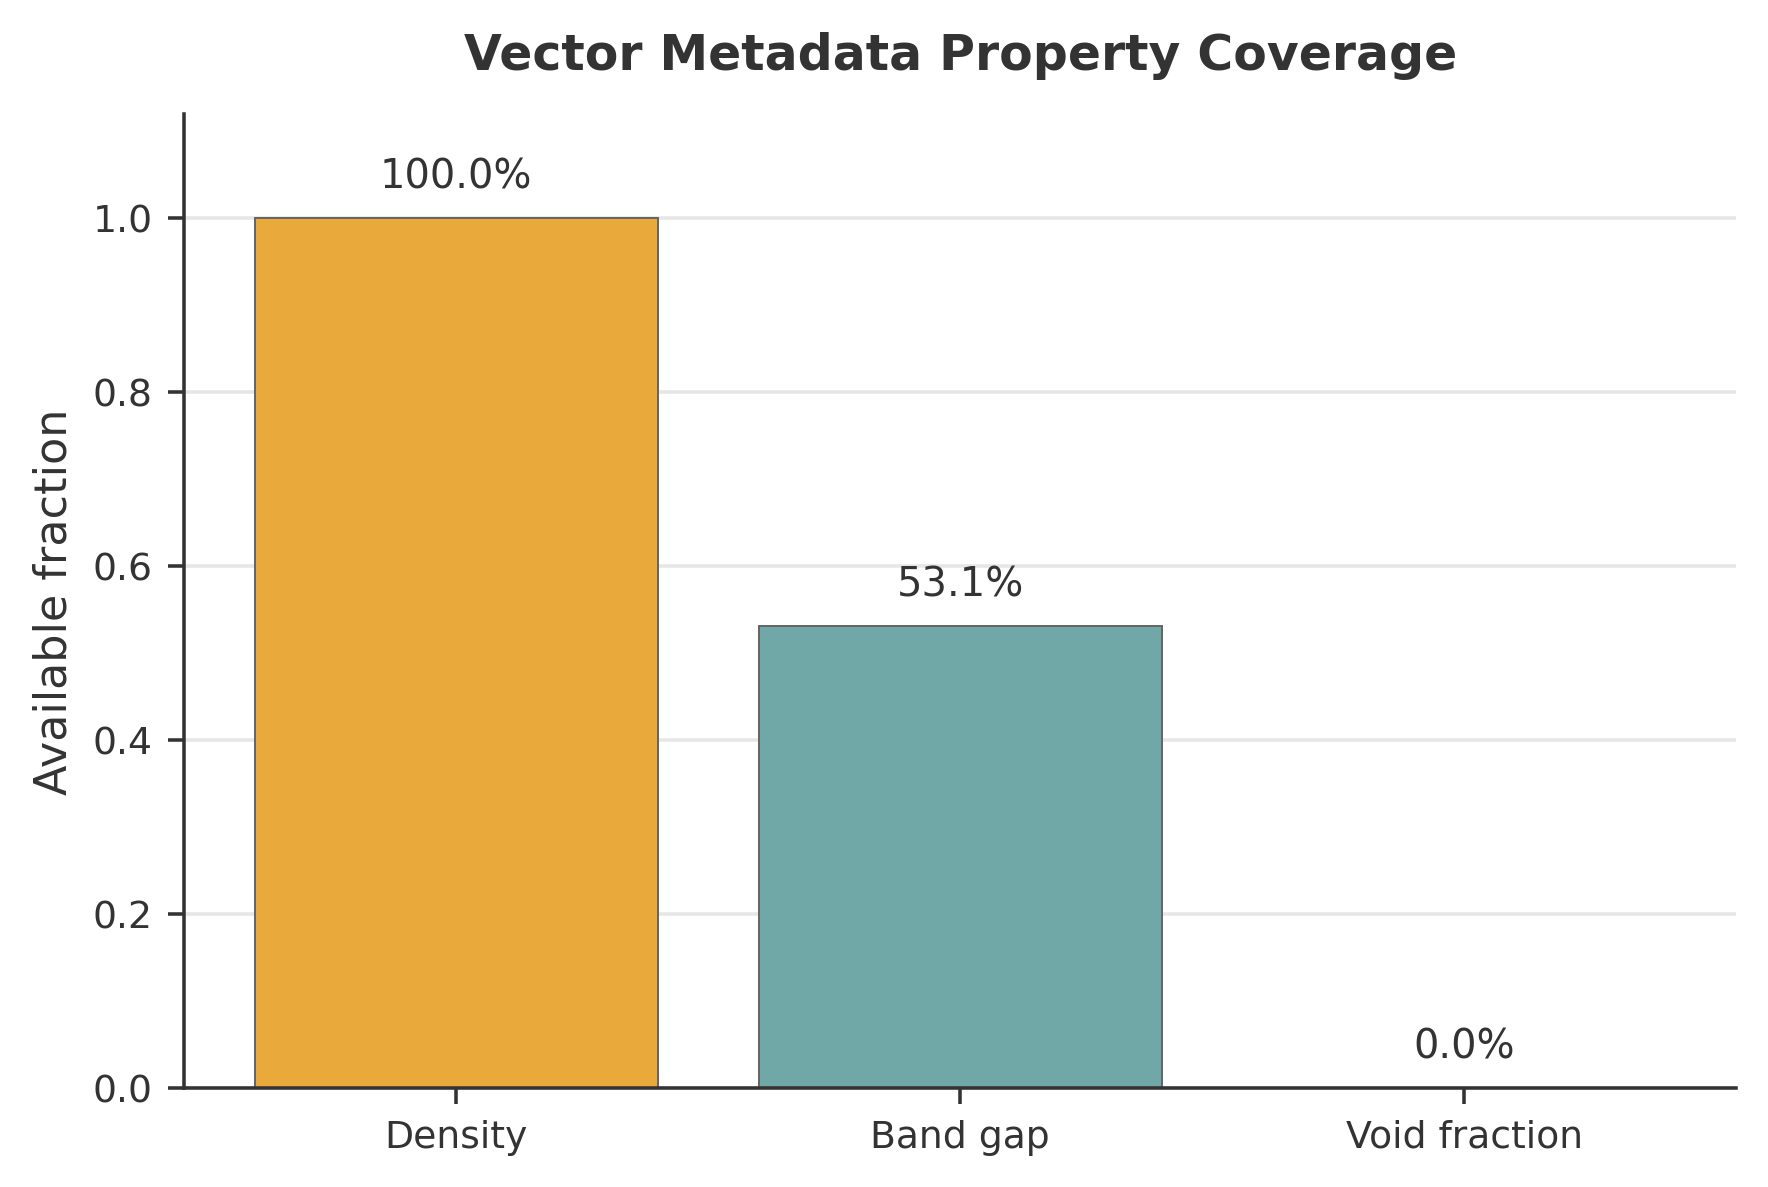
\includegraphics[width=0.6\linewidth]{figures/figure_2_data_coverage.png}
  \caption{Coverage of metadata fields used in the current reproducible QMOF-Rec evaluation. Density is available for all records, band gap is partially available, and void fraction is absent.}
  \label{fig:coverage}
\end{figure}

The missing void-fraction field materially affects interpretation. The current evaluation supports density-aware and partial band-gap-aware ranking. It does not support strong porosity-aware, adsorption-specific, or CO$_2$ uptake claims. CO$_2$ adsorption recommendations should be read as preliminary recommendation behavior under incomplete metadata, not as validated adsorption screening.

Five query scenarios are evaluated: CO$_2$ adsorption, photocatalysis, lightweight storage, balanced screening, and insulating frameworks. Each query/seed uses a shared pool of 100 records and $K=5$. Seeds 42--51 vary tie-breaking and stochastic search within five scenarios. The semantic signal is an engineered query-dependent proxy; this is not an evaluation of the deployed embedding retriever. Table~\ref{tab:ranking} compares the primary methods and the added DE portfolio comparator. Table~\ref{tab:ablation} contains distinct component diagnostics, with LEA repeated only as a reference. The supplement reports all scenario-level outcomes, joint sensitivity, runtime dispersion and scaling, and descriptor-level checks.

%% ════════════════════════════════════════════════════════════════════════════
\section{Recommendation Evaluation Metrics}
\label{sec:metrics}

\subsection{Offline Recommendation Protocol Without User Histories}

Because no historical user-click or rating log exists for QMOF materials, the evaluation follows an offline query-driven recommendation protocol. QMOF-Rec is a hybrid scientific recommender with a strong content-based focus: it does not rely on collaborative filtering because no large-scale user--MOF interaction log is available. The task is similar to session-based or context-aware recommendation, where the query supplies the current user intent and item content supplies the ranking evidence. User feedback is included architecturally for future online learning, but the present evaluation uses query-dependent objective weights rather than user ratings.

\subsection{Ranking, Diversity, and Coverage Metrics}
\label{sec:metrics_detail}

Mean relevance is computed as
\begin{equation}
  \mathrm{Rel}@K(S_K) = \frac{1}{K}\sum_{m_i \in S_K} R(m_i, q).
\end{equation}
If binary or graded expert labels become available, Precision@$K$ can be computed as $\mathrm{Precision}@K(S_K) = \frac{1}{K}\sum_{m_i\in S_K}\mathbf{1}[\mathrm{rel}(m_i,q)\geq\theta]$, where $\theta$ is a relevance threshold. In the current offline protocol, no expert-labeled relevant set is available, so Precision@$K$ is defined as a future supervised recommender-system metric. Discounted cumulative gain is
\begin{equation}
  \mathrm{DCG}@K = \sum_{r=1}^{K}\frac{2^{\mathrm{rel}_r}-1}{\log_2(r+1)},
\end{equation}
where $\mathrm{rel}_r=R(m_{(r)},q)$ is the same masked utility used by WeightedSum. The ideal list sorts that utility within the identical candidate pool. Therefore WeightedSum maximizes Rel@$K$ and this NDCG by construction; a tie indicates utility preservation, not independent relevance accuracy. Normalized discounted cumulative gain is $\mathrm{NDCG}@K = \mathrm{DCG}@K / \mathrm{IDCG}@K$. The final rerun keeps relevance scoring on the mask-aware active utility vector, but computes intra-list diversity (ILD) over a full-precision hybrid material representation containing observed density, observed band gap, formula-derived descriptors, and formula-derived metadata proxies:
\begin{equation}
  \mathrm{ILD}_{\mathrm{hybrid}}(S_K) = \frac{2}{K(K-1)}\sum_{i<j}d_{\mathrm{hybrid}}(\mathbf{h}_i,\mathbf{h}_j).
\end{equation}
The hybrid distance masks missing physical dimensions, excludes void fraction, and uses full precision before any manuscript rounding. This representation is used for final diversity, ParetoCrowding crowding distance, MMR redundancy, and LEA list-level diversity. Unique@$K$ is the fraction of unique items within a top-$K$ list and is distinct from catalog coverage.
Catalog coverage measures how much of the item space is recommended across a query set $\mathcal{Q}$:
\begin{equation}
  \mathrm{Coverage} = \frac{\left|\bigcup_{q\in\mathcal{Q}}S_K(q)\right|}{|\mathcal{M}|}.
\end{equation}
The ablation rerun also reports Unique@$K$ within each recommendation list. Runtime is reported as mean runtime in milliseconds. The reported hypervolume value is a hypervolume proxy rather than exact Pareto hypervolume, computed per list as $\mathrm{Rel}@5\times\mathrm{ILD}\times\overline{s}_{\mathrm{gap}}\times\overline{s}_{\mathrm{density}}\times\overline{s}_{\mathrm{stability}}$, then averaged over runs; it is a comparative proxy only.

All ranking results below were regenerated with the final diversity-aware, mask-aware implementation, the configuration in \path{configs/final_diversity_aware_masked_protocol.json}, and shared candidate pools for all ranking methods. Source hashes and the successful reproduction gate are recorded in the reviewer-revision artifacts. Historical artifact directories were absent from the authoritative checkout; no missing historical run is represented as reproduced.

%% ════════════════════════════════════════════════════════════════════════════
\section{Recommendation Performance: Ranking Quality and Portfolio Diversity}
\label{sec:results}

The final protocol reproduces all seven original methods' Rel@5, NDCG@5, and diversity values to four decimal places. LEA preserves the same utility as WeightedSum and has modestly higher hybrid diversity. ParetoCrowding, MMR, SemanticOnly, and Random all exceed LEA diversity in the original comparison; only MMR preserves the maximum utility among these four. Table~\ref{tab:ranking} adds a differential-evolution (DE) portfolio baseline on the same pools and representation.

\begin{table}[H]\centering\small
\caption{Reproduced ranking results and the added DE portfolio baseline; five scenarios, ten seeds, shared pools of 100, $K=5$. MMR stops after five selections and exactly matches the original full-ranking top five in all 50 runs. Runtime includes method-specific preprocessing, excludes catalog scoring and retrieval, and is a mean; dispersion is in the supplement. The product-based HV proxy is not Pareto hypervolume.}\label{tab:ranking}
\begin{tabular}{lrrrrr}
\toprule
Method & Rel@5 & Diversity & NDCG@5 & HV proxy & ms\\\midrule
WeightedSum & 0.8479 & 0.0187 & 1.0000 & 0.0121 & 0.05\\
LEA & 0.8479 & 0.0224 & 1.0000 & 0.0141 & 87.26\\
TOPSIS & 0.8479 & 0.0187 & 1.0000 & 0.0121 & 1.13\\
ParetoCrowding & 0.8447 & 0.0263 & 0.9952 & 0.0125 & 224.68\\
MMR (top-5) & 0.8479 & 0.0241 & 1.0000 & 0.0150 & 12.70\\
Random & 0.7695 & 0.0237 & 0.8809 & 0.0067 & 0.05\\
SemanticOnly & 0.7600 & 0.0240 & 0.8678 & 0.0057 & 0.04\\
DE portfolio & 0.8479 & 0.0242 & 1.0000 & 0.0149 & 69.39\\
\bottomrule\end{tabular}\end{table}

The DE comparator uses the differential-evolution method of Storn and Price \cite{storn1997}, implemented in SciPy 1.13.1 \cite{scipyde}, with 30 random-key vectors over the 100 candidates and 1,800 list-objective evaluations (initial population plus 59 generations). The five largest keys select five distinct records. One initial member encodes WeightedSum's top five and the other 29 are random. The fixed portfolio utility is $\overline R+0.10\overline B+0.10\mathrm{ILD}-0.05\exp(-\mathrm{ILD})$. Selected items are ordered by masked relevance. This is an additional portfolio-search baseline, not an exact implementation of LEA's changing candidate-level fitness; equal evaluation counts do not imply equal computational work. Distance preparation is included in its reported runtime. No tuning against external outcomes is performed.

The original MMR routine completed all 100 ranks before taking the first five. Its reproduced mean runtime was 2209.67 ms, versus 87.26 ms for LEA. Stopping the unchanged MMR selection rule at five returns identical lists in all 50 cases and takes 12.70 ms. The historical speed advantage of LEA therefore reflects unequal output work and is withdrawn. LEA is intermediate in diversity between WeightedSum and MMR, but the matched top-five workload does not support recommending it for a runtime advantage.

\begin{figure}[H]\centering
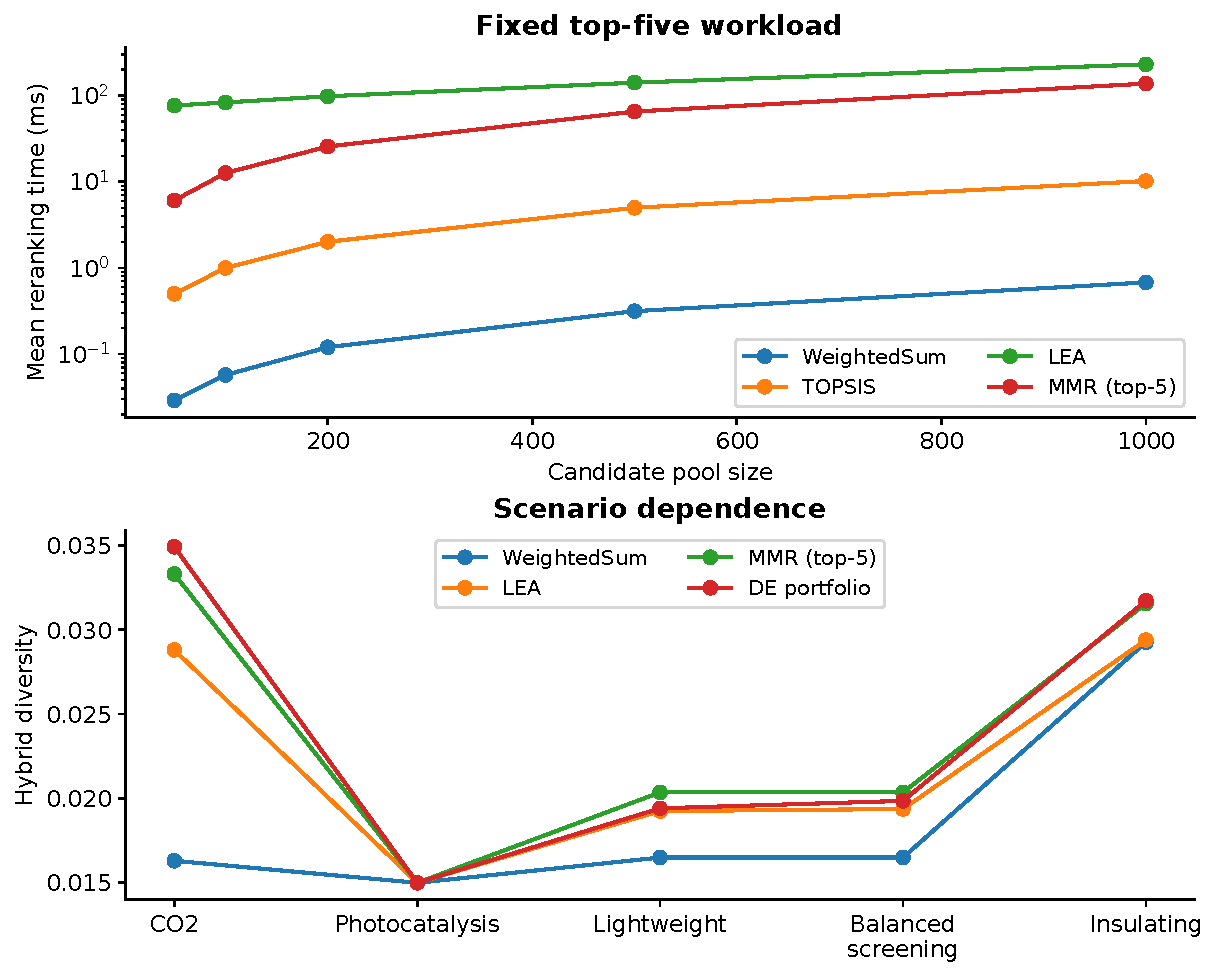
\includegraphics[width=\linewidth]{figures/runtime_scenarios_readable.pdf}
\caption{Reranking scalability at fixed $K=5$ and scenario-dependent hybrid diversity. Timing uses five scenarios, three seeds, and three repeats per setting; it excludes catalog scoring, embedding retrieval, network calls, and generation.}
\label{fig:runtime}\end{figure}

\subsection{Example Recommendation Scenarios}

Table~\ref{tab:examples} reports the highest-ranked LEA recommendation for each evaluated query scenario from the final diversity-aware, mask-aware rerun. These examples illustrate the recommendation use case and should be read as offline recommendation outputs, not as experimentally validated application-performance results.

For CO$_2$ adsorption, the recommender balances query relevance, density, and stability-oriented signals while excluding porosity from numerical ranking because void fraction is unavailable; the missing void-fraction descriptor limits adsorption-specific interpretation. For photocatalysis, the recommender emphasizes semantic relevance and band-gap suitability. For lightweight storage, low density and list diversity are central. For balanced screening, the goal is broad multi-objective suitability rather than a single target. For insulating frameworks, the top-$K$ list prioritizes wide band gap and stability-oriented signals.

\begin{table}[H]
\centering
\caption{Example LEA top-1 recommendations from the final diversity-aware, mask-aware QMOF-Rec rerun. Void-fraction values are unavailable in the current metadata. The LEA utility is a weighted optimization score and is not a probability or a quantity constrained to $[0,1]$.}
\label{tab:examples}
\scriptsize
\setlength{\tabcolsep}{3pt}
\begin{tabular}{L{2.2cm} L{2.0cm} L{3.25cm} C{1.25cm} C{1.2cm} C{1.35cm} L{2.1cm}}
\toprule
\textbf{Scenario} & \textbf{QMOF ID} & \textbf{Formula} & \textbf{Band gap} & \textbf{Density} & \textbf{LEA score} & \textbf{Rationale}\\
\midrule
CO$_2$ adsorption  & qmof-82fb334 & Co$_2$C$_{22}$H$_{16}$N$_4$O$_{10}$ & 2.754 & 1.773 & 0.8471 & Relevance, density, stability\\
Photocatalysis     & qmof-13a76dd & Zn$_4$C$_{40}$H$_{28}$N$_{12}$O$_8$ & 3.309 & 0.983 & 0.9597 & Query match, band gap\\
Lightweight storage & qmof-13a76dd & Zn$_4$C$_{40}$H$_{28}$N$_{12}$O$_8$ & 3.309 & 0.983 & 1.0056 & Low density, relevance\\
Balanced screening  & qmof-13a76dd & Zn$_4$C$_{40}$H$_{28}$N$_{12}$O$_8$ & 3.309 & 0.983 & 0.9827 & Broad objective profile\\
Insulating frameworks & qmof-4050181 & Li$_4$C$_{28}$H$_{32}$N$_4$O$_8$ & 5.066 & 0.936 & 0.8686 & Wide band gap, stability\\
\bottomrule
\end{tabular}
\end{table}

%% ════════════════════════════════════════════════════════════════════════════
\section{Audit of Graph-Related Evidence}
\label{sec:gnn}

The authoritative checkout contains the final ranking runner and backend graph-related modules, but the available GAT module is not a trained or evaluated implementation within the final ranking protocol and the final runner uses engineered proxy scores. The former graph property-prediction values and graph topology counts cannot be regenerated by this protocol. They are withdrawn from the revised results rather than carried forward as verified measurements. This does not establish that graph learning is ineffective; it restricts the evidence to the executable experiment.
\begin{table}[H]\centering\small
\caption{Scope of the graph-related evidence in the authoritative executable repository.}\label{tab:gnn}
\begin{tabular}{p{3.1cm}p{10.3cm}}
\toprule
Component & Executable evidence\\\midrule
Proxy S/A & Hand-crafted formula, density, and band-gap scores\\
GNN ranking & No trained GNN is called by the final protocol\\
CIF structures & Present on disk; unused in final ranking\\
Prior regression table & Not independently reproduced; numerical claims withdrawn\\
\bottomrule\end{tabular}\end{table}


\section{Component Ablations and Metadata-Proxy Augmentation}
\label{sec:ablation}


\begin{table}[H]\centering\small
\caption{Component diagnostics. LEA is repeated as the reference; principal baselines appear only in Table~\ref{tab:ranking}. True no diversity sets both $\gamma=0$ and redundancy coefficient $\lambda=0$. Proxy variants are engineered metadata augmentation. The uniform-pool diagnostic changes candidate generation and is not a same-pool ranking comparison.}\label{tab:ablation}
\begin{tabular}{lrrrr}
\toprule
Variant & Rel@5 & NDCG@5 & Diversity & ms\\\midrule
LEA & 0.8479 & 1.0000 & 0.0224 & 87.26\\
LEA $\gamma=0$ only & 0.8479 & 1.0000 & 0.0224 & 86.27\\
LEA true no diversity & 0.8479 & 1.0000 & 0.0187 & 84.07\\
LEA no self-clean & 0.8479 & 1.0000 & 0.0224 & 85.30\\
Proxy-S scoring & 0.8479 & 1.0000 & 0.0205 & 0.04\\
Proxy-A scoring & 0.8479 & 1.0000 & 0.0160 & 0.04\\
LEA + proxy S & 0.8479 & 1.0000 & 0.0205 & 84.86\\
LEA + proxy A & 0.8479 & 1.0000 & 0.0158 & 85.33\\
Zero-imputed WeightedSum & 0.8479 & 1.0000 & 0.0187 & 0.10\\
LEA uniform pool & 0.8154 & 0.9981 & 0.0264 & 84.56\\
\bottomrule\end{tabular}\end{table}
The historical ``no diversity'' row set only $\gamma=0$ while retaining $\lambda=0.05$ in $-\lambda e^{-D}$. It is now labeled ``gamma=0 only.'' Disabling both terms changes mean diversity from 0.0224 to 0.0187, showing that the two diversity-dependent terms must be distinguished. The gamma-only and no-self-cleaning variants retain the baseline aggregate metrics. This result supports an effect of the retained redundancy term under this implementation, not a universal advantage of the named optimizer. The zero-imputation diagnostic changes scoring on the same pools and evaluates selections using the original masked utility. Uniform-pool LEA tests the engineered candidate generator, not a trained retrieval model.

\section{Scenario-Level Analysis and Coefficient Sensitivity}
\label{sec:stats}

The independent descriptive units are five query scenarios; ten seeds per scenario measure repeated algorithm behavior and do not create 50 independent scientific tasks. The LEA--WeightedSum diversity differences are 0.0125, 0.0000, 0.0028, 0.0029, and 0.0001 for CO$_2$, photocatalysis, lightweight, balanced, and insulating scenarios. The CO$_2$ scenario contributes approximately 68\% of the sum of these differences. We therefore report scenario dependence and no statistical superiority claim. Complete per-scenario results for all primary methods are given in Supplementary Table~S1.

The joint sweep uses gamma values 0, 0.025, 0.05, 0.10, 0.20, 0.40, and 0.80, and redundancy coefficients 0, 0.025, 0.05, 0.10, and 0.20 on all 50 query/seed pools: 1,750 runs. We define observable activation by a changed top-five set, order, or unrounded metric; a nonzero coefficient alone is not evidence of an output effect. Coefficients are retained at their predefined baseline, not selected from the sweep. The supplement reports every coefficient pair and scenario-level evidence, including null effects. Numerical fitness histories are also hashed in the artifacts.

\begin{table}[H]\centering\small
\caption{Gamma sensitivity with redundancy coefficient fixed at 0.05. Changed sets are relative to baseline gamma=0.10.}\label{tab:gamma}
\begin{tabular}{rrrr}
\toprule
$\gamma$ & Rel@5 & Diversity & Changed sets\\\midrule
0 & 0.8479 & 0.0224 & 0/50\\
0.025 & 0.8479 & 0.0224 & 0/50\\
0.05 & 0.8479 & 0.0224 & 0/50\\
0.1 & 0.8479 & 0.0224 & 0/50\\
0.2 & 0.8479 & 0.0224 & 0/50\\
0.4 & 0.8479 & 0.0224 & 0/50\\
0.8 & 0.8478 & 0.0225 & 1/50\\
\bottomrule\end{tabular}\end{table}

\begin{figure}[H]\centering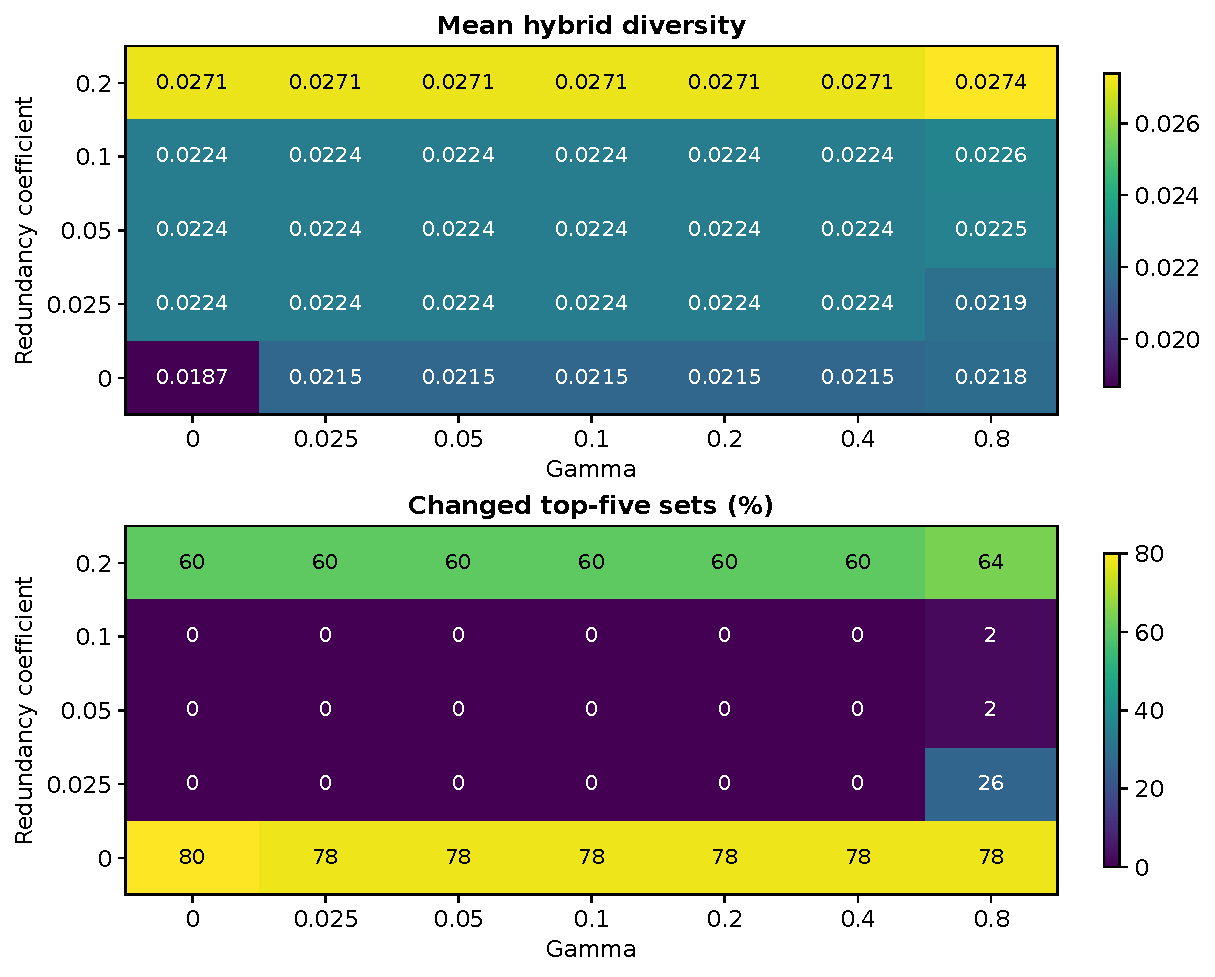
\includegraphics[width=\linewidth]{figures/sensitivity_readable.pdf}
\caption{Joint coefficient sensitivity. The upper panel reports diversity; the lower panel reports changed top-five sets relative to baseline. Changing the selected set is distinguished from changing the reported mean utility.}\label{fig:sensitivity}\end{figure}


\section{Auxiliary Explanation: Template Audit and Limits}
\label{sec:rag_eval}

Explanation is an auxiliary interface module; it has no effect on candidate generation, objective weights, or rankings in this benchmark. The reproduced runner emits 30 deterministic templates conditioned on seed-42 LEA candidate identifiers. It checks identifier presence and limitation phrases, but directly assigns metadata consistency, the nominal explanation-quality score, and all unsupported-claim flags. Those assigned values cannot demonstrate factual accuracy or a zero hallucination rate. We withdraw the former quality-score table as an independent evaluation and report the executable check scope instead.

\begin{table}[H]\centering\small
\caption{Actual scope of the deterministic explanation routine.}\label{tab:rag_results}
\begin{tabular}{p{5.0cm}p{8.4cm}}
\toprule
Output/check & Interpretation\\\midrule
30 candidate-conditioned templates & Reproducible local output; no live LLM call\\
Identifier inclusion & String-presence check against selected IDs\\
Limitation wording & Template/phrase check\\
Metadata and violation scores & Assigned in code; not independent measurements\\
Expert usefulness and faithfulness & Not evaluated\\
\bottomrule\end{tabular}\end{table}
A future explanation benchmark requires independent claim checking, source attribution, expert ratings, and adversarial prompts. The interface screenshots in the supplement illustrate historical UI behavior only.

\section{Runtime, Scalability, and Descriptor-Level Screening}
\label{sec:robustness}

Reranking time was measured for WeightedSum, TOPSIS, LEA, and top-five MMR at pool sizes 50, 100, 200, 500, and 1,000, using five scenarios, seeds 42--44, and three repeats (45 measurements per method/size). These are serial wall-clock timings on one machine and exclude shared catalog scoring and retrieval. Mean and standard deviation, plus the raw measurements, are supplied in the supplement and artifacts. At fixed $K$, top-five MMR avoids the cubic distance-work growth of the original full-list scalar loop; its distance comparisons scale as $O(nK^2)$ in this implementation. LEA repeatedly remaps population vectors against the pool, with dominant work proportional to population size times iterations times pool size and objective dimension. These measurements establish local post-retrieval scaling only.

Descriptor-level screening compares catalog, candidate-pool, Random, WeightedSum, and LEA distributions for observed density and band gap, including missingness and prespecified bands. Because these descriptors also affect candidate generation and utility, their shifts are consistency checks, not independent discovery validation. Density thresholds are not porosity or uptake measurements; a favorable band gap alone does not demonstrate photocatalytic activity. The mean LEA shortlist density in the lightweight scenario is 0.890 g/cm$^3$, versus 1.696 in the catalog. Mean observed gaps are 2.804 eV for photocatalysis and 4.311 eV for insulating frameworks; all selected insulating gaps are at least 3.5 eV. These shifts support consistency with those descriptor-level intents, but not independent application performance. In the lightweight candidate pools, only 7 of 100 gaps are observed; selection favors those observed gaps, illustrating a completeness effect as well as a density preference.

\section{Discussion}
\label{sec:discussion}

The evidence supports an auditable screening formulation under incomplete metadata, with established algorithms as components. Relevance and NDCG are aligned with the utility that WeightedSum optimizes, so their ties cannot validate scientific relevance independently. Full-precision hybrid distances resolve variation hidden by binned objectives, but the resulting diversity remains representation-dependent and partly heuristic.

LEA sits between WeightedSum and MMR in the original aggregate diversity comparison, with much of its difference concentrated in one scenario. The corrected ablation identifies a contribution from diversity-dependent fitness, chiefly the retained redundancy term at the baseline setting; gamma-only and self-cleaning ablations do not establish separate benefits. The added DE portfolio comparator broadens the optimization comparison but uses a fixed list objective, whereas LEA retains history-dependent candidate fitness. Neither comparison proves universal algorithm superiority.

The corrected top-five MMR is faster than LEA while preserving the higher original diversity and equal relevance. Accordingly, a runtime-based ``middle ground'' argument is not supported by the matched workload. The original ratio is retained only as an implementation audit, not as evidence for choosing LEA.

Learned atomistic GNNs and transformers answer a different representation-learning question from the present engineered-proxy benchmark. A fair learned comparison needs matched inputs, training splits, checkpoints, and targets. Although CIFs exist locally, the final protocol supplies none of these trained ranking comparisons. Bayesian optimization and active learning additionally require a sequential acquisition task and an oracle or held-out property target; the current deterministic utility is not such validation. These remain explicit gaps rather than artificial comparison rows.

\section{Limitations}
\label{sec:limitations}

Only five engineered query scenarios, $K=5$, incomplete descriptors, heuristic stability, and deterministic semantic proxies are evaluated. Band gap and density influence both selection and evaluation. The engineered metadata-proxy block retains a zero fallback for missing band gap and is not fully mask-pure even though the physical coordinate is masked. No independent adsorption, synthesis, porosity, expert relevance, new DFT, online-user, or generative-discovery validation is provided. The metadata-proxy augmentation rows are engineered scores, not trained GNN predictions. Historical property-prediction numbers were not reproducible from the authoritative final protocol and are excluded. Explanation templates and assigned flags cannot establish LLM faithfulness. DE and LEA optimize differently defined utilities, and the limited search budget and query suite do not establish general optimizer rankings. Timing excludes retrieval, catalog scoring, and generation, and should not be read as production latency.

\section{Future Work}
\label{sec:future}

Future work should rebuild the full QMOF descriptor matrix, add real embedding-based retrieval evaluation, incorporate CIF-derived graph embeddings, evaluate graph-aware recommendation on larger query suites, assess LLM faithfulness and citation fidelity with expert review, expand comparisons with evolutionary and swarm-based baselines such as NSGA-II, PSO, and GA, add Bayesian optimization as a separate model-based sequential optimization baseline, evaluate additional MMR settings, and optimize deployment latency.

Recommender-system extensions should include expert-labeled relevance benchmarks, user studies with materials scientists, active-learning from feedback, preference-aware recommendation for application domains, cold-start analysis for newly added QMOFs, learning-to-rank baselines, and explainable-recommendation evaluation with faithfulness and usefulness metrics. Live RAG/LLM extensions should include multi-turn dialogue evaluation, citation fidelity scoring, expert usefulness ratings, and adversarial robustness testing against fabrication-inducing prompts.

%% ════════════════════════════════════════════════════════════════════════════
\section{Conclusion}
\label{sec:conclusion}

QMOF-Rec provides a reproducible formulation for ranking existing QMOF records under incomplete metadata. The authoritative final protocol reproduces the reported primary ranking values. The revision adds complete scenario-level results, joint coefficient sensitivity, a true no-diversity ablation, a differential-evolution portfolio baseline, matched top-five timing and scalability, and descriptor-level screening checks. These tests support careful separation of masked utility, material diversity, and physical validation. They do not establish LEA as the core novelty or preferred optimizer: top-five MMR preserves its diversity advantage and runs faster in the corrected comparison. Learned graph models and independently evaluated LLM explanations remain future extensions; the present evidence consists of metadata-based screening and deterministic templates.

\section*{Declarations}

\noindent\textbf{Data Availability.}\ The public QMOF database is available from the original QMOF data release. The evaluation uses locally prepared QMOF-derived vector metadata and processed artifacts generated from the repository scripts. The processed metadata and frozen result CSVs are included in the accompanying versioned reproducibility archive \path{qmof-rec-v1.1-COMMT-revision.tar.gz}. The baseline source repository is: \url{https://github.com/MehrdadJalali-AI/qmof-rec}.

\noindent\textbf{Code Availability.}\ The baseline source repository is linked below. The reviewer-revision code and machine-readable evidence are packaged in the accompanying versioned reproducibility archive \path{qmof-rec-v1.1-COMMT-revision.tar.gz}: \url{https://github.com/MehrdadJalali-AI/qmof-rec}.

\noindent\textbf{Demo Availability.}\ A live interactive demonstration of the QMOF-Rec user interface is available at \url{https://qmofrecsystem.netlify.app/}. The deployment is provided solely as an interface demonstration and does not replace the offline ranking experiments, metadata-proxy analyses, coefficient sensitivity studies, or deterministic explanation-template audit reported in this manuscript.

\noindent\textbf{Use of Generative AI.}\ Generative AI tools were used to assist with language editing, consistency checking, code-review support, figure-preparation support, and response-to-review preparation. The authors are responsible for reviewing and approving the final text, code changes, figures, response materials, and scientific conclusions before submission.

\noindent\textbf{Competing Interests.}\ The authors declare no competing interests.

\noindent\textbf{Author Contributions (CRediT).}\ Soumya Sekhar Banerjee: Software, Investigation, Visualization, Writing---original draft. Arnd Koeppe: Methodology, Writing---review \& editing, including critical evaluation of the recommendation and validation framework and interpretation of the analyses. Mehrdad Jalali: Conceptualization, Methodology, Supervision, Writing---original draft, Writing---review \& editing.

\noindent\textbf{Funding.}\ The authors received no specific funding for this work.

\noindent\textbf{Acknowledgements.}\ The authors thank SRH University of Applied Sciences Heidelberg for institutional support.

%% ════════════════════════════════════════════════════════════════════════════
\begin{thebibliography}{99}

\bibitem{adomavicius2011} G.~Adomavicius and Y.~Kwon. New recommendation techniques for multicriteria rating systems. \textit{IEEE Intelligent Systems}, 26(5):48--55, 2011.

\bibitem{burke2002} R.~Burke. Hybrid recommender systems: Survey and experiments. \textit{User Modeling and User-Adapted Interaction}, 12:331--370, 2002.

\bibitem{carbonell1998} J.~Carbonell and J.~Goldstein. The use of MMR, diversity-based reranking for reordering documents and producing summaries. In \textit{Proc.\ 21st ACM SIGIR}, pp.\ 335--336, 1998.

\bibitem{chen2019} C.~Chen, W.~Ye, Y.~Zuo, C.~Zheng, and S.~P.~Ong. Graph networks as a universal machine learning framework for molecules and crystals. \textit{Chemistry of Materials}, 31(9):3564--3572, 2019.

\bibitem{dalirinia2024} E.~Dalirinia, M.~Jalali, M.~Yaghoobi, and H.~Tabatabaee. Lotus effect optimization algorithm (LEA): a lotus nature-inspired algorithm for engineering design optimization. \textit{The Journal of Supercomputing}, 80:8543--8597, 2024.

\bibitem{deb2002} K.~Deb, A.~Pratap, S.~Agarwal, and T.~Meyarivan. A fast and elitist multiobjective genetic algorithm: NSGA-II. \textit{IEEE Trans.\ Evolutionary Computation}, 6(2):182--197, 2002.

\bibitem{hamilton2017} W.~L.~Hamilton, R.~Ying, and J.~Leskovec. Inductive representation learning on large graphs. In \textit{Advances in Neural Information Processing Systems}, vol.\ 30, 2017.

\bibitem{hwang1981} C.-L.~Hwang and K.~Yoon. \textit{Multiple Attribute Decision Making: Methods and Applications}. Springer, 1981.

\bibitem{jalali2023} M.~Jalali, M.~Schmitt, A.~D.~Dinga~Wonanke, C.~W\"{o}ll, and P.~Friederich. MOFGalaxyNet: a social network analysis for predicting guest accessibility in metal--organic frameworks utilizing graph convolutional networks. \textit{Journal of Cheminformatics}, 15:99, 2023.

\bibitem{jalali2025lens} M.~Jalali, B.~Vu, S.~Mehraeen, S.~Chandna, and F.~Jalali. MOF-LENS: Bio-inspired lotus effect optimization for accelerated discovery of metal--organic framework nanocarriers for doxorubicin delivery in cancer therapy. \textit{Materials Today Communications}, 49:114448, 2025.

\bibitem{jalali2025bh} M.~Jalali, A.~D.~Dinga~Wonanke, P.~Friederich, and C.~W\"{o}ll. The black hole strategy: Gravity-based representative sampling for frugal graph learning on metal--organic framework networks. \textit{Journal of Chemical Information and Modeling}, 65(20):10885--10902, 2025.

\bibitem{jannach2014} D.~Jannach, M.~Zanker, and M.~Fuchs. Leveraging multi-criteria customer feedback for satisfaction analysis and improved recommendations. \textit{Information Technology \& Tourism}, 14:119--149, 2014.

\bibitem{johnson2019} J.~Johnson, M.~Douze, and H.~J\'{e}gou. Billion-scale similarity search with GPUs. \textit{IEEE Transactions on Big Data}, 7(3):535--547, 2019.

\bibitem{kipf2017} T.~N.~Kipf and M.~Welling. Semi-supervised classification with graph convolutional networks. In \textit{International Conference on Learning Representations}, 2017.

\bibitem{lewis2020} P.~Lewis et al. Retrieval-augmented generation for knowledge-intensive NLP tasks. In \textit{Advances in Neural Information Processing Systems}, vol.\ 33, pp.\ 9459--9474, 2020.

\bibitem{lops2011} P.~Lops, M.~de~Gemmis, and G.~Semeraro. Content-based recommender systems: State of the art and trends. In \textit{Recommender Systems Handbook}, pp.\ 73--105. Springer, 2011.

\bibitem{luo2023} Y.~Luo, K.~Yan, and S.~Ji. MOFormer: Self-supervised transformer model for metal--organic framework property prediction. \textit{Journal of the American Chemical Society}, 145(3):1615--1624, 2023.

\bibitem{reimers2019} N.~Reimers and I.~Gurevych. Sentence-BERT: Sentence embeddings using siamese BERT-networks. In \textit{Proc.\ EMNLP-IJCNLP}, pp.\ 3982--3992, 2019.

\bibitem{ricci2011} F.~Ricci, L.~Rokach, B.~Shapira, and P.~B.~Kantor (eds). \textit{Recommender Systems Handbook}. Springer, 2011.

\bibitem{rosen2021} A.~S.~Rosen et al. Machine learning the quantum-chemical properties of metal--organic frameworks for accelerated materials discovery. \textit{Matter}, 4(5):1578--1597, 2021.

\bibitem{rosen2022} A.~S.~Rosen et al. High-throughput predictions of metal--organic framework electronic properties: theoretical challenges, graph neural networks, and data exploration. \textit{npj Computational Materials}, 8:112, 2022.

\bibitem{seko2018} A.~Seko, H.~Hayashi, H.~Kashima, and I.~Tanaka. Matrix- and tensor-based recommender systems for the discovery of currently unknown inorganic compounds. \textit{Physical Review Materials}, 2:013805, 2018.

\bibitem{shahriari2016} B.~Shahriari et al. Taking the human out of the loop: A review of Bayesian optimization. \textit{Proceedings of the IEEE}, 104(1):148--175, 2016.

\bibitem{qu2023} J.~Qu, Y.~R.~Xie, K.~M.~Ciesielski, C.~E.~Porter, E.~S.~Toberer, and E.~Ertekin. Leveraging language representation for materials exploration and discovery. \textit{npj Computational Materials}, 10:58, 2024. doi:10.1038/s41524-024-01231-8.

\bibitem{kadiassistant2026} A.~Cierpka, M.~S.~Islam, J.~Steinh\"{u}lb, E.~D.~S.~Domtchoueng, M.~Selzer, and A.~Koeppe. KadiAssistant: A conversational AI agent for information retrieval in Kadi4Mat. arXiv:2605.18850, 2026.

\bibitem{velickovic2018} P.~Veli\v{c}kovi\'{c} et al. Graph attention networks. In \textit{International Conference on Learning Representations}, 2018.

\bibitem{xie2018} T.~Xie and J.~C.~Grossman. Crystal graph convolutional neural networks for an accurate and interpretable prediction of material properties. \textit{Physical Review Letters}, 120:145301, 2018.

\bibitem{zhang2020} Y.~Zhang and X.~Chen. Explainable recommendation: A survey and new perspectives. \textit{Foundations and Trends in Information Retrieval}, 14(1):1--101, 2020.

\bibitem{storn1997} R.~Storn and K.~Price. Differential Evolution---A Simple and Efficient Heuristic for Global Optimization over Continuous Spaces. \textit{Journal of Global Optimization}, 11:341--359, 1997. doi:10.1023/A:1008202821328.

\bibitem{scipyde} SciPy developers. Differential evolution, SciPy 1.13.1 reference manual. \url{https://docs.scipy.org/doc/scipy-1.13.1/reference/generated/scipy.optimize.differential_evolution.html}.
\end{thebibliography}

\end{document}
